% Options for packages loaded elsewhere
\PassOptionsToPackage{unicode}{hyperref}
\PassOptionsToPackage{hyphens}{url}
%
\documentclass[
  9pt,
  ignorenonframetext,
  aspectratio=169]{beamer}
\usepackage{pgfpages}
\setbeamertemplate{caption}[numbered]
\setbeamertemplate{caption label separator}{: }
\setbeamercolor{caption name}{fg=normal text.fg}
\beamertemplatenavigationsymbolsempty
% Prevent slide breaks in the middle of a paragraph
\widowpenalties 1 10000
\raggedbottom
\setbeamertemplate{part page}{
  \centering
  \begin{beamercolorbox}[sep=16pt,center]{part title}
    \usebeamerfont{part title}\insertpart\par
  \end{beamercolorbox}
}
\setbeamertemplate{section page}{
  \centering
  \begin{beamercolorbox}[sep=12pt,center]{part title}
    \usebeamerfont{section title}\insertsection\par
  \end{beamercolorbox}
}
\setbeamertemplate{subsection page}{
  \centering
  \begin{beamercolorbox}[sep=8pt,center]{part title}
    \usebeamerfont{subsection title}\insertsubsection\par
  \end{beamercolorbox}
}
\AtBeginPart{
  \frame{\partpage}
}
\AtBeginSection{
  \ifbibliography
  \else
    \frame{\sectionpage}
  \fi
}
\AtBeginSubsection{
  \frame{\subsectionpage}
}
\usepackage{lmodern}
\usepackage{amssymb,amsmath}
\usepackage{ifxetex,ifluatex}
\ifnum 0\ifxetex 1\fi\ifluatex 1\fi=0 % if pdftex
  \usepackage[T1]{fontenc}
  \usepackage[utf8]{inputenc}
  \usepackage{textcomp} % provide euro and other symbols
\else % if luatex or xetex
  \usepackage{unicode-math}
  \defaultfontfeatures{Scale=MatchLowercase}
  \defaultfontfeatures[\rmfamily]{Ligatures=TeX,Scale=1}
\fi
\usetheme[]{Berkeley}
\usecolortheme{dove}
\usefonttheme{structurebold}
% Use upquote if available, for straight quotes in verbatim environments
\IfFileExists{upquote.sty}{\usepackage{upquote}}{}
\IfFileExists{microtype.sty}{% use microtype if available
  \usepackage[]{microtype}
  \UseMicrotypeSet[protrusion]{basicmath} % disable protrusion for tt fonts
}{}
\makeatletter
\@ifundefined{KOMAClassName}{% if non-KOMA class
  \IfFileExists{parskip.sty}{%
    \usepackage{parskip}
  }{% else
    \setlength{\parindent}{0pt}
    \setlength{\parskip}{6pt plus 2pt minus 1pt}}
}{% if KOMA class
  \KOMAoptions{parskip=half}}
\makeatother
\usepackage{xcolor}
\IfFileExists{xurl.sty}{\usepackage{xurl}}{} % add URL line breaks if available
\IfFileExists{bookmark.sty}{\usepackage{bookmark}}{\usepackage{hyperref}}
\hypersetup{
  pdftitle={Análise de variância e correlação},
  pdfauthor={Frederico Bertholini},
  hidelinks,
  pdfcreator={LaTeX via pandoc}}
\urlstyle{same} % disable monospaced font for URLs
\newif\ifbibliography
\usepackage{color}
\usepackage{fancyvrb}
\newcommand{\VerbBar}{|}
\newcommand{\VERB}{\Verb[commandchars=\\\{\}]}
\DefineVerbatimEnvironment{Highlighting}{Verbatim}{commandchars=\\\{\}}
% Add ',fontsize=\small' for more characters per line
\usepackage{framed}
\definecolor{shadecolor}{RGB}{248,248,248}
\newenvironment{Shaded}{\begin{snugshade}}{\end{snugshade}}
\newcommand{\AlertTok}[1]{\textcolor[rgb]{0.94,0.16,0.16}{#1}}
\newcommand{\AnnotationTok}[1]{\textcolor[rgb]{0.56,0.35,0.01}{\textbf{\textit{#1}}}}
\newcommand{\AttributeTok}[1]{\textcolor[rgb]{0.77,0.63,0.00}{#1}}
\newcommand{\BaseNTok}[1]{\textcolor[rgb]{0.00,0.00,0.81}{#1}}
\newcommand{\BuiltInTok}[1]{#1}
\newcommand{\CharTok}[1]{\textcolor[rgb]{0.31,0.60,0.02}{#1}}
\newcommand{\CommentTok}[1]{\textcolor[rgb]{0.56,0.35,0.01}{\textit{#1}}}
\newcommand{\CommentVarTok}[1]{\textcolor[rgb]{0.56,0.35,0.01}{\textbf{\textit{#1}}}}
\newcommand{\ConstantTok}[1]{\textcolor[rgb]{0.00,0.00,0.00}{#1}}
\newcommand{\ControlFlowTok}[1]{\textcolor[rgb]{0.13,0.29,0.53}{\textbf{#1}}}
\newcommand{\DataTypeTok}[1]{\textcolor[rgb]{0.13,0.29,0.53}{#1}}
\newcommand{\DecValTok}[1]{\textcolor[rgb]{0.00,0.00,0.81}{#1}}
\newcommand{\DocumentationTok}[1]{\textcolor[rgb]{0.56,0.35,0.01}{\textbf{\textit{#1}}}}
\newcommand{\ErrorTok}[1]{\textcolor[rgb]{0.64,0.00,0.00}{\textbf{#1}}}
\newcommand{\ExtensionTok}[1]{#1}
\newcommand{\FloatTok}[1]{\textcolor[rgb]{0.00,0.00,0.81}{#1}}
\newcommand{\FunctionTok}[1]{\textcolor[rgb]{0.00,0.00,0.00}{#1}}
\newcommand{\ImportTok}[1]{#1}
\newcommand{\InformationTok}[1]{\textcolor[rgb]{0.56,0.35,0.01}{\textbf{\textit{#1}}}}
\newcommand{\KeywordTok}[1]{\textcolor[rgb]{0.13,0.29,0.53}{\textbf{#1}}}
\newcommand{\NormalTok}[1]{#1}
\newcommand{\OperatorTok}[1]{\textcolor[rgb]{0.81,0.36,0.00}{\textbf{#1}}}
\newcommand{\OtherTok}[1]{\textcolor[rgb]{0.56,0.35,0.01}{#1}}
\newcommand{\PreprocessorTok}[1]{\textcolor[rgb]{0.56,0.35,0.01}{\textit{#1}}}
\newcommand{\RegionMarkerTok}[1]{#1}
\newcommand{\SpecialCharTok}[1]{\textcolor[rgb]{0.00,0.00,0.00}{#1}}
\newcommand{\SpecialStringTok}[1]{\textcolor[rgb]{0.31,0.60,0.02}{#1}}
\newcommand{\StringTok}[1]{\textcolor[rgb]{0.31,0.60,0.02}{#1}}
\newcommand{\VariableTok}[1]{\textcolor[rgb]{0.00,0.00,0.00}{#1}}
\newcommand{\VerbatimStringTok}[1]{\textcolor[rgb]{0.31,0.60,0.02}{#1}}
\newcommand{\WarningTok}[1]{\textcolor[rgb]{0.56,0.35,0.01}{\textbf{\textit{#1}}}}
\usepackage{graphicx}
\makeatletter
\def\maxwidth{\ifdim\Gin@nat@width>\linewidth\linewidth\else\Gin@nat@width\fi}
\def\maxheight{\ifdim\Gin@nat@height>\textheight\textheight\else\Gin@nat@height\fi}
\makeatother
% Scale images if necessary, so that they will not overflow the page
% margins by default, and it is still possible to overwrite the defaults
% using explicit options in \includegraphics[width, height, ...]{}
\setkeys{Gin}{width=\maxwidth,height=\maxheight,keepaspectratio}
% Set default figure placement to htbp
\makeatletter
\def\fps@figure{htbp}
\makeatother
\setlength{\emergencystretch}{3em} % prevent overfull lines
\providecommand{\tightlist}{%
  \setlength{\itemsep}{0pt}\setlength{\parskip}{0pt}}
\setcounter{secnumdepth}{5}

\title{Análise de variância e correlação}
\subtitle{Métodos Quantitativos Aplicados à Ciência Política}
\author{Frederico Bertholini}
\date{07.dez.2020}

\begin{document}
\frame{\titlepage}

\begin{frame}[allowframebreaks]
  \tableofcontents[hideallsubsections]
\end{frame}
\hypertarget{formalizando-hipuxf3teses}{%
\section{Formalizando Hipóteses}\label{formalizando-hipuxf3teses}}

\begin{frame}{Um caso comum - Esta análise está correta?}
\protect\hypertarget{um-caso-comum---esta-anuxe1lise-estuxe1-correta}{}
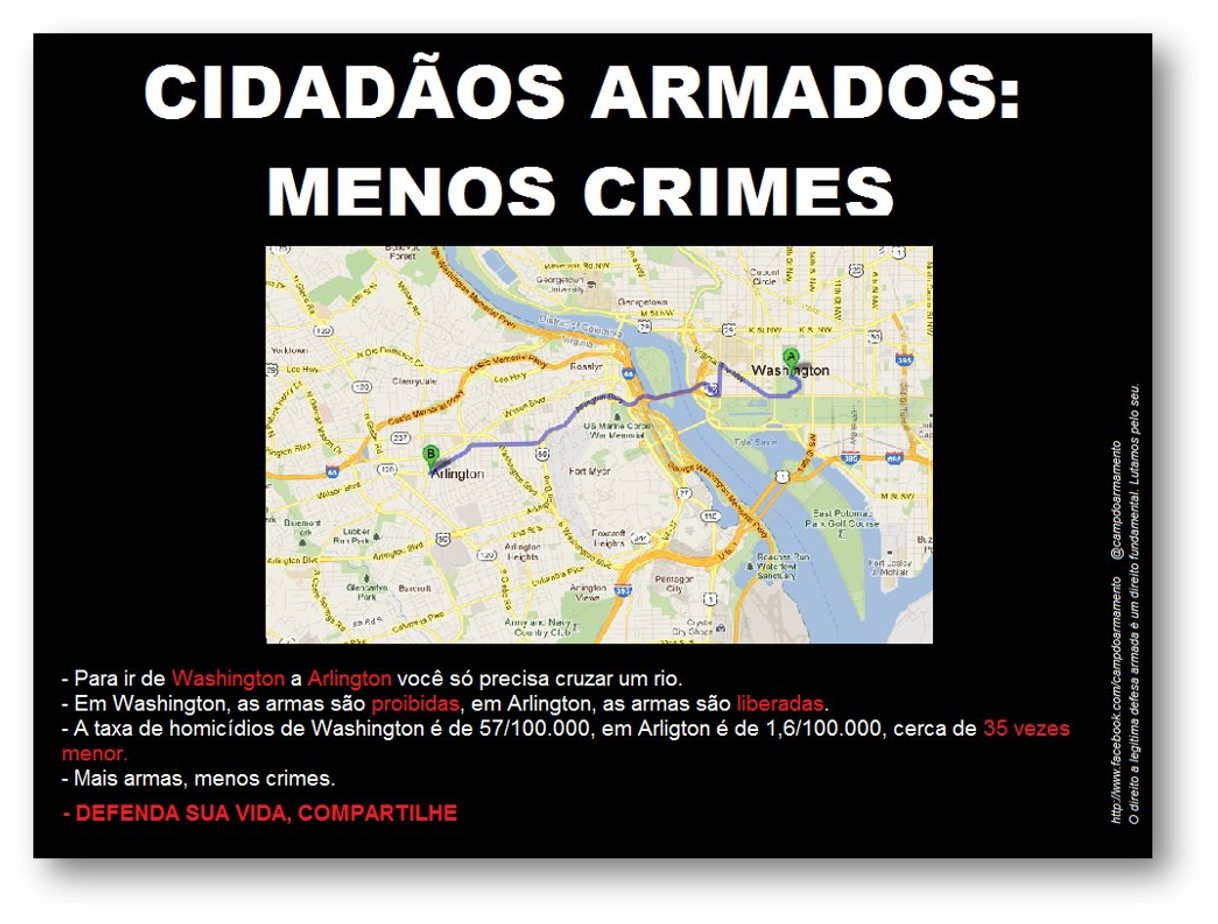
\includegraphics{imgs/armas_crime.png}
\end{frame}

\begin{frame}{Comparação de médias}
\protect\hypertarget{comparauxe7uxe3o-de-muxe9dias}{}
A resposta é não. (por quê?)

Em todo caso, ela ilustra uma situação bem comum na prática, onde se
deseja comparar médias. No caso, deseja-se comparar as taxas médias de
mortalidade em cidades onde as armas são proibidas ou liberadas.
Deseja-se testar se a média de homicídios em cidades onde armas são
liberadas é menor que a média de homicídios em cidades onde armas são
proibidas. (Como você colheria dados para esse estudo?)

As hipóteses, portanto, são:

\(H_0:\mu_L=\mu_P\)

\(H_A:\mu_L<\mu_P\)
\end{frame}

\begin{frame}[fragile]{Lembrando a base de trabalho}
\protect\hypertarget{lembrando-a-base-de-trabalho}{}
\begin{Shaded}
\begin{Highlighting}[]
\KeywordTok{summary}\NormalTok{(dfe }\OperatorTok{\%\textgreater{}\%}\StringTok{ }\NormalTok{dplyr}\OperatorTok{::}\KeywordTok{select}\NormalTok{(}\OperatorTok{{-}}\NormalTok{id))}
\end{Highlighting}
\end{Shaded}

\begin{verbatim}
     media           faltas         turma               idade      
 Min.   :40.00   Min.   : 0.00   Length:60          Min.   :18.00  
 1st Qu.:70.00   1st Qu.: 2.00   Class :character   1st Qu.:19.75  
 Median :73.75   Median : 4.00   Mode  :character   Median :22.00  
 Mean   :74.38   Mean   : 4.25                      Mean   :25.23  
 3rd Qu.:80.00   3rd Qu.: 6.00                      3rd Qu.:29.00  
 Max.   :95.00   Max.   :10.00                      Max.   :49.00  
       interess        tempocup                  escola       estcivil 
 Secundário:24   não tem   : 4   Tudo privada       :20   Casado  :17  
 Principal :34   até 2h    : 3   Maior parte privada:15   Solteiro:42  
 NA's      : 2   de 2h a 4h:11   Maior parte pública:18   NA's    : 1  
                 de 4h a 6h:42   Tudo pública       : 7                
                 + de 6h   : 0                                         
                                                                       
     nota1           nota2      
 Min.   :40.00   Min.   :40.00  
 1st Qu.:67.88   1st Qu.:71.75  
 Median :72.00   Median :77.00  
 Mean   :72.26   Mean   :76.49  
 3rd Qu.:78.00   3rd Qu.:82.12  
 Max.   :94.00   Max.   :97.00  
\end{verbatim}
\end{frame}

\begin{frame}{Diferença entre médias (amostras não pareadas)}
\protect\hypertarget{diferenuxe7a-entre-muxe9dias-amostras-nuxe3o-pareadas}{}
\(H_0:\text{A média de notas de casados e solteiros é igual}\) ou
\(H_0:\mu_c-\mu_s=0\) ou \(H_0:\mu_c = \mu_s\)

\(H_1:\text{A média de notas de casados e solteiros é diferente}\) ou
\(H_1:\mu_c-\mu_s \neq 0\) ou \(H_1:\mu_c \neq \mu_s\)

Variável \textbf{dependente}: Notas

Variável \textbf{independente}: Situação conjugal

O que eu quero testar? Se a situação conjugal \emph{faz diferença} na
nota.

É \textbf{efeito}? Não! (Pearl, 2020) Inferência vs.~Causalidade
\end{frame}

\begin{frame}[fragile]{Como testar na prática? Distribuições:}
\protect\hypertarget{como-testar-na-pruxe1tica-distribuiuxe7uxf5es}{}
\begin{Shaded}
\begin{Highlighting}[]
\NormalTok{dfe }\OperatorTok{\%\textgreater{}\%}\StringTok{ }\KeywordTok{drop\_na}\NormalTok{(estcivil) }\OperatorTok{\%\textgreater{}\%}\StringTok{ }
\StringTok{  }\KeywordTok{ggplot}\NormalTok{(}\KeywordTok{aes}\NormalTok{(}\DataTypeTok{fill=}\NormalTok{estcivil,}\DataTypeTok{x=}\NormalTok{media,}\DataTypeTok{color=}\NormalTok{estcivil,}\DataTypeTok{group=}\NormalTok{estcivil)) }\OperatorTok{+}
\StringTok{  }\KeywordTok{geom\_density}\NormalTok{(}\DataTypeTok{color=}\OtherTok{NA}\NormalTok{,}\DataTypeTok{alpha=}\NormalTok{.}\DecValTok{65}\NormalTok{) }\OperatorTok{+}\StringTok{  }
\StringTok{  }\KeywordTok{geom\_vline}\NormalTok{(}\DataTypeTok{data=}\NormalTok{. }\OperatorTok{\%\textgreater{}\%}\StringTok{ }\KeywordTok{group\_by}\NormalTok{(estcivil) }\OperatorTok{\%\textgreater{}\%}\StringTok{ }\KeywordTok{summarise}\NormalTok{(}\DataTypeTok{media=}\KeywordTok{mean}\NormalTok{(media,}\DataTypeTok{na.rm =}\NormalTok{ T)),}
             \DataTypeTok{size=}\DecValTok{2}\NormalTok{,}\KeywordTok{aes}\NormalTok{(}\DataTypeTok{xintercept=}\NormalTok{media,}\DataTypeTok{color=}\NormalTok{estcivil)) }\OperatorTok{+}\StringTok{ }
\StringTok{  }\KeywordTok{guides}\NormalTok{(}\DataTypeTok{color=}\StringTok{"none"}\NormalTok{) }\OperatorTok{+}\StringTok{ }\NormalTok{theme\_ipsum\_mod}
\end{Highlighting}
\end{Shaded}

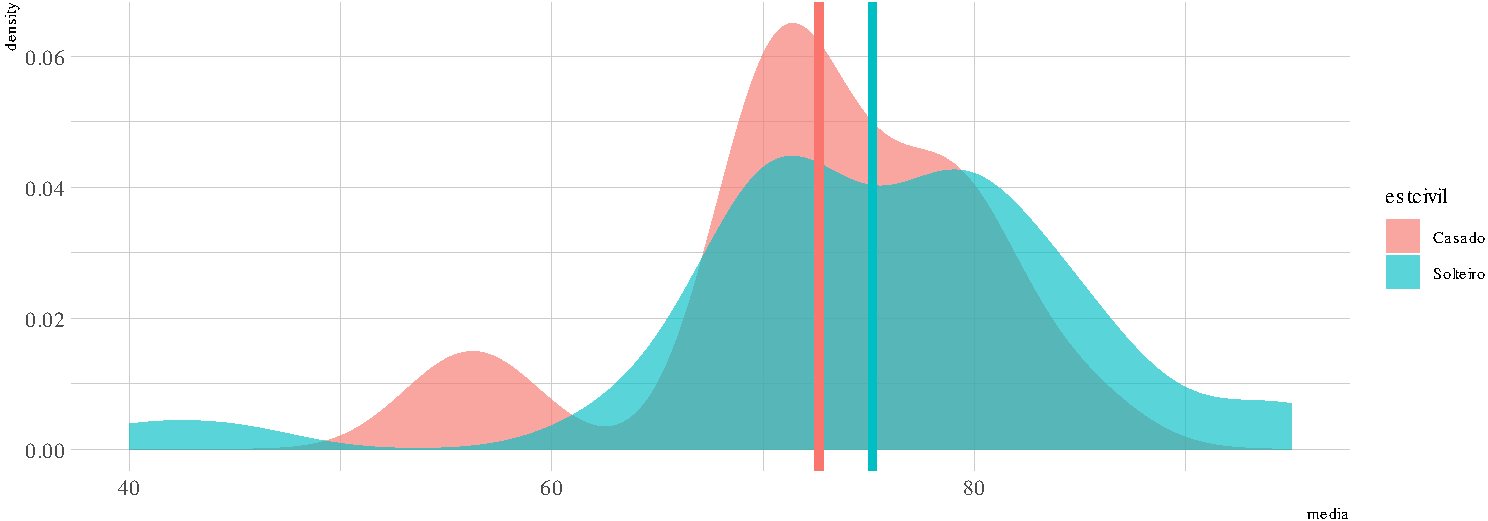
\includegraphics{aula_11_files/figure-beamer/unnamed-chunk-2-1.pdf}
\end{frame}

\begin{frame}[fragile]{Como testar na prática? Vamos construir
intervalos}
\protect\hypertarget{como-testar-na-pruxe1tica-vamos-construir-intervalos}{}
\begin{Shaded}
\begin{Highlighting}[]
\NormalTok{dfe }\OperatorTok{\%\textgreater{}\%}\StringTok{ }\KeywordTok{drop\_na}\NormalTok{(estcivil) }\OperatorTok{\%\textgreater{}\%}\StringTok{ }
\StringTok{  }\KeywordTok{ggplot}\NormalTok{(}\KeywordTok{aes}\NormalTok{(}\DataTypeTok{fill=}\NormalTok{estcivil,}\DataTypeTok{x=}\NormalTok{media,}\DataTypeTok{color=}\NormalTok{estcivil,}\DataTypeTok{y=}\NormalTok{estcivil)) }\OperatorTok{+}
\StringTok{  }\KeywordTok{stat\_summary}\NormalTok{(}\DataTypeTok{fun=}\NormalTok{mean, }\DataTypeTok{geom=}\StringTok{"point"}\NormalTok{) }\OperatorTok{+}\StringTok{ }
\StringTok{  }\KeywordTok{stat\_summary}\NormalTok{(}\DataTypeTok{fun.data=}\NormalTok{mean\_ci, }\DataTypeTok{geom=}\StringTok{"errorbar"}\NormalTok{, }\DataTypeTok{width=}\FloatTok{0.2}\NormalTok{) }\OperatorTok{+}
\StringTok{  }\KeywordTok{geom\_vline}\NormalTok{(}\DataTypeTok{data=}\NormalTok{. }\OperatorTok{\%\textgreater{}\%}\StringTok{ }\KeywordTok{group\_by}\NormalTok{(estcivil) }\OperatorTok{\%\textgreater{}\%}\StringTok{ }\KeywordTok{summarise}\NormalTok{(}\DataTypeTok{media=}\KeywordTok{mean}\NormalTok{(media,}\DataTypeTok{na.rm =}\NormalTok{ T)),}
             \DataTypeTok{size=}\DecValTok{2}\NormalTok{,}\KeywordTok{aes}\NormalTok{(}\DataTypeTok{xintercept=}\NormalTok{media,}\DataTypeTok{color=}\NormalTok{estcivil)) }\OperatorTok{+}\StringTok{ }
\StringTok{  }\NormalTok{theme\_ipsum\_mod }\OperatorTok{+}\KeywordTok{theme}\NormalTok{(}\DataTypeTok{legend.position =} \StringTok{"none"}\NormalTok{)}
\end{Highlighting}
\end{Shaded}

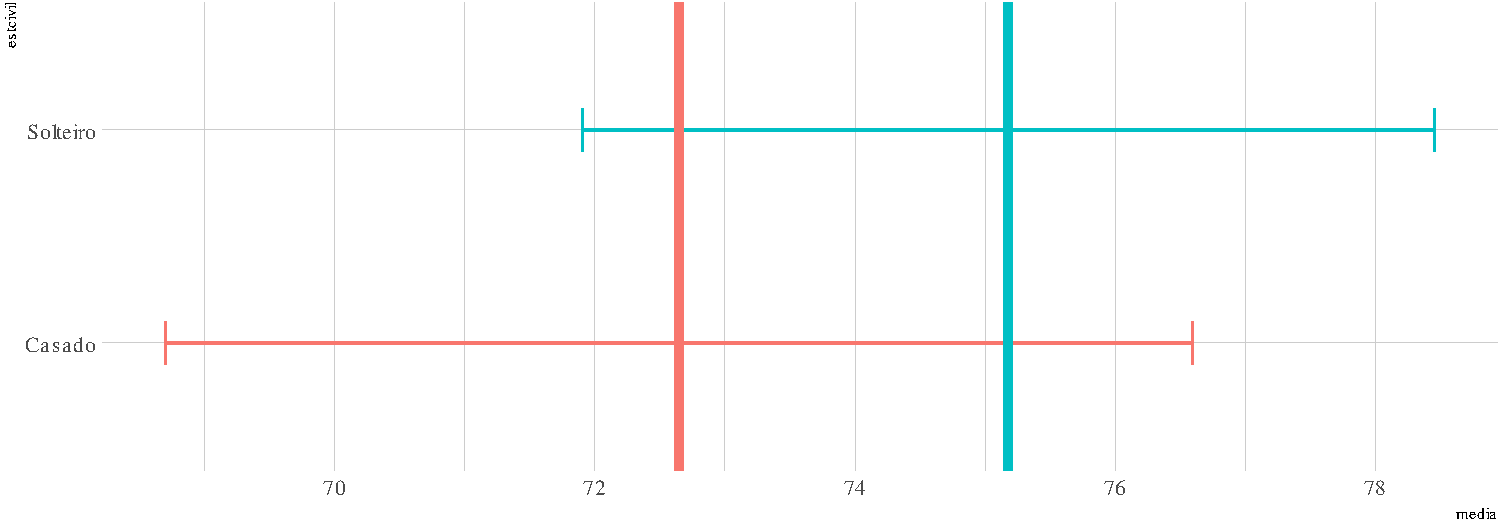
\includegraphics{aula_11_files/figure-beamer/unnamed-chunk-3-1.pdf}
\end{frame}

\begin{frame}[fragile]{Como testar na prática? Teste-t}
\protect\hypertarget{como-testar-na-pruxe1tica-teste-t}{}
\begin{Shaded}
\begin{Highlighting}[]
\NormalTok{t\_test\_results \textless{}{-}}\StringTok{ }\NormalTok{dfe }\OperatorTok{\%\textgreater{}\%}
\StringTok{  }\KeywordTok{t\_test}\NormalTok{(}\DataTypeTok{formula =}\NormalTok{ media }\OperatorTok{\textasciitilde{}}\StringTok{ }\NormalTok{estcivil,}
         \DataTypeTok{order =} \KeywordTok{c}\NormalTok{(}\StringTok{"Casado"}\NormalTok{, }\StringTok{"Solteiro"}\NormalTok{))}
\NormalTok{t\_test\_results}
\end{Highlighting}
\end{Shaded}

\begin{verbatim}
# A tibble: 1 x 6
  statistic  t_df p_value alternative lower_ci upper_ci
      <dbl> <dbl>   <dbl> <chr>          <dbl>    <dbl>
1     -1.03  40.4   0.311 two.sided      -7.52     2.46
\end{verbatim}
\end{frame}

\begin{frame}{Outro exercício}
\protect\hypertarget{outro-exercuxedcio}{}
\(H_0:\mu_\text{3joan} = \mu_\text{3joad}\)

\(H_1:\mu_\text{3joan} \neq \mu_\text{3joad}\)

Variável \textbf{dependente}: Notas

Variável \textbf{independente}: Turma (apenas 3joan e 3joad)
\end{frame}

\begin{frame}[fragile]{Intervalos}
\protect\hypertarget{intervalos}{}
\begin{Shaded}
\begin{Highlighting}[]
\NormalTok{dfe }\OperatorTok{\%\textgreater{}\%}\StringTok{ }\NormalTok{dplyr}\OperatorTok{::}\KeywordTok{filter}\NormalTok{(turma }\OperatorTok{\%in\%}\StringTok{ }\KeywordTok{c}\NormalTok{(}\StringTok{"3joan"}\NormalTok{,}\StringTok{"3joad"}\NormalTok{)) }\OperatorTok{\%\textgreater{}\%}\StringTok{ }
\StringTok{  }\KeywordTok{ggplot}\NormalTok{(}\KeywordTok{aes}\NormalTok{(}\DataTypeTok{fill=}\NormalTok{turma,}\DataTypeTok{x=}\NormalTok{media,}\DataTypeTok{color=}\NormalTok{turma,}\DataTypeTok{y=}\NormalTok{turma)) }\OperatorTok{+}
\StringTok{  }\KeywordTok{stat\_summary}\NormalTok{(}\DataTypeTok{fun=}\NormalTok{mean, }\DataTypeTok{geom=}\StringTok{"point"}\NormalTok{) }\OperatorTok{+}\StringTok{ }
\StringTok{  }\KeywordTok{stat\_summary}\NormalTok{(}\DataTypeTok{fun.data=}\NormalTok{mean\_ci, }\DataTypeTok{geom=}\StringTok{"errorbar"}\NormalTok{,}\DataTypeTok{width=}\FloatTok{0.2}\NormalTok{) }\OperatorTok{+}
\StringTok{  }\KeywordTok{geom\_vline}\NormalTok{(}\DataTypeTok{data=}\NormalTok{. }\OperatorTok{\%\textgreater{}\%}\StringTok{ }\KeywordTok{group\_by}\NormalTok{(turma) }\OperatorTok{\%\textgreater{}\%}\StringTok{ }\KeywordTok{summarise}\NormalTok{(}\DataTypeTok{media=}\KeywordTok{mean}\NormalTok{(media,}\DataTypeTok{na.rm =}\NormalTok{ T)),}
             \DataTypeTok{size=}\DecValTok{2}\NormalTok{,}\KeywordTok{aes}\NormalTok{(}\DataTypeTok{xintercept=}\NormalTok{media,}\DataTypeTok{color=}\NormalTok{turma)) }\OperatorTok{+}\StringTok{ }
\StringTok{  }\NormalTok{theme\_ipsum\_mod }\OperatorTok{+}\KeywordTok{theme}\NormalTok{(}\DataTypeTok{legend.position =} \StringTok{"none"}\NormalTok{)}
\end{Highlighting}
\end{Shaded}

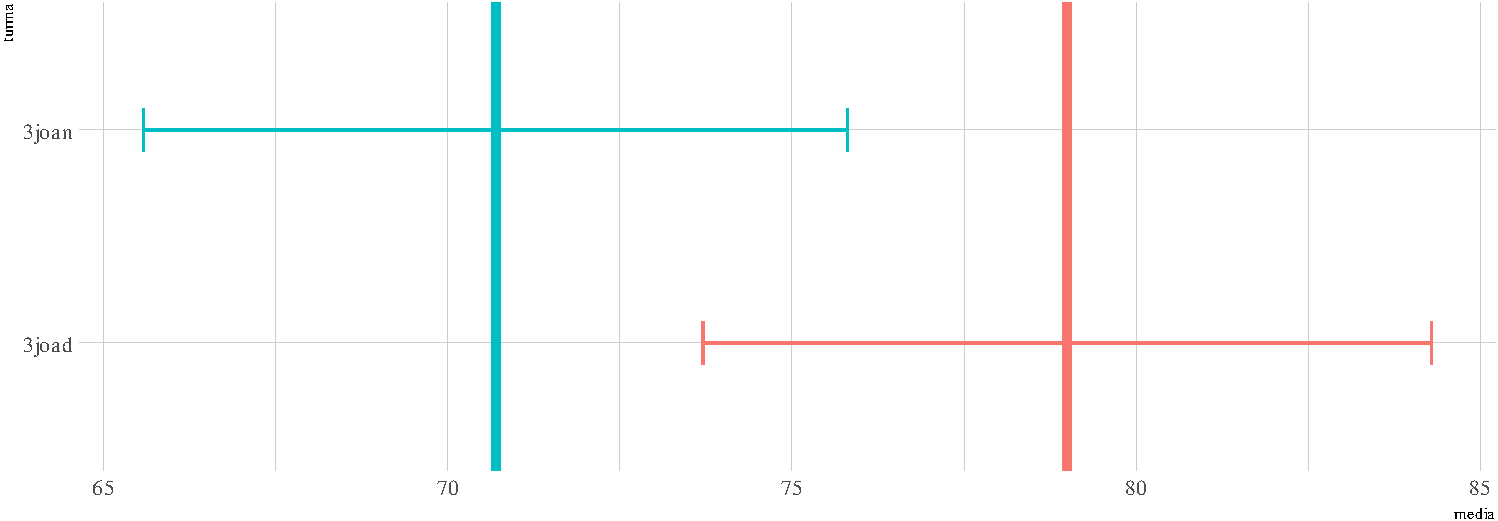
\includegraphics{aula_11_files/figure-beamer/unnamed-chunk-5-1.pdf}
\end{frame}

\begin{frame}[fragile]{Como testar na prática? Teste-t}
\protect\hypertarget{como-testar-na-pruxe1tica-teste-t-1}{}
\begin{Shaded}
\begin{Highlighting}[]
\NormalTok{t\_test\_results \textless{}{-}}\StringTok{ }\NormalTok{dfe }\OperatorTok{\%\textgreater{}\%}\StringTok{ }
\StringTok{  }\NormalTok{dplyr}\OperatorTok{::}\KeywordTok{filter}\NormalTok{(turma }\OperatorTok{\%in\%}\StringTok{ }\KeywordTok{c}\NormalTok{(}\StringTok{"3joan"}\NormalTok{,}\StringTok{"3joad"}\NormalTok{)) }\OperatorTok{\%\textgreater{}\%}\StringTok{ }
\StringTok{  }\KeywordTok{t\_test}\NormalTok{(}\DataTypeTok{formula =}\NormalTok{ media }\OperatorTok{\textasciitilde{}}\StringTok{ }\NormalTok{turma)}
\NormalTok{t\_test\_results}
\end{Highlighting}
\end{Shaded}

\begin{verbatim}
# A tibble: 1 x 6
  statistic  t_df p_value alternative lower_ci upper_ci
      <dbl> <dbl>   <dbl> <chr>          <dbl>    <dbl>
1      2.37  36.0  0.0232 two.sided       1.20     15.4
\end{verbatim}
\end{frame}

\begin{frame}[fragile]{Olhando no infer graficamente}
\protect\hypertarget{olhando-no-infer-graficamente}{}
\begin{Shaded}
\begin{Highlighting}[]
\CommentTok{\# calculate the observed statistic}
\NormalTok{media\_turmas \textless{}{-}}\StringTok{ }\NormalTok{dfe }\OperatorTok{\%\textgreater{}\%}\StringTok{ }
\StringTok{  }\NormalTok{dplyr}\OperatorTok{::}\KeywordTok{filter}\NormalTok{(turma }\OperatorTok{\%in\%}\StringTok{ }\KeywordTok{c}\NormalTok{(}\StringTok{"3joan"}\NormalTok{,}\StringTok{"3joad"}\NormalTok{)) }\OperatorTok{\%\textgreater{}\%}\StringTok{ }
\StringTok{  }\KeywordTok{specify}\NormalTok{(media }\OperatorTok{\textasciitilde{}}\StringTok{ }\NormalTok{turma) }\OperatorTok{\%\textgreater{}\%}
\StringTok{  }\KeywordTok{calculate}\NormalTok{(}\DataTypeTok{stat =} \StringTok{"t"}\NormalTok{, }\DataTypeTok{order =} \KeywordTok{c}\NormalTok{(}\StringTok{"3joan"}\NormalTok{,}\StringTok{"3joad"}\NormalTok{))}

\CommentTok{\# generate the null distribution with the theoretical t}
\NormalTok{distribuicao\_teorica \textless{}{-}}\StringTok{ }\NormalTok{dfe }\OperatorTok{\%\textgreater{}\%}\StringTok{ }
\StringTok{  }\NormalTok{dplyr}\OperatorTok{::}\KeywordTok{filter}\NormalTok{(turma }\OperatorTok{\%in\%}\StringTok{ }\KeywordTok{c}\NormalTok{(}\StringTok{"3joan"}\NormalTok{,}\StringTok{"3joad"}\NormalTok{)) }\OperatorTok{\%\textgreater{}\%}\StringTok{ }
\StringTok{  }\KeywordTok{specify}\NormalTok{(media }\OperatorTok{\textasciitilde{}}\StringTok{ }\NormalTok{turma) }\OperatorTok{\%\textgreater{}\%}
\StringTok{  }\KeywordTok{hypothesize}\NormalTok{(}\DataTypeTok{null =} \StringTok{"independence"}\NormalTok{) }\OperatorTok{\%\textgreater{}\%}
\StringTok{  }\KeywordTok{calculate}\NormalTok{(}\DataTypeTok{stat =} \StringTok{"t"}\NormalTok{, }\DataTypeTok{order =} \KeywordTok{c}\NormalTok{(}\StringTok{"3joan"}\NormalTok{,}\StringTok{"3joad"}\NormalTok{))}
\end{Highlighting}
\end{Shaded}
\end{frame}

\begin{frame}[fragile]{Visualizando}
\protect\hypertarget{visualizando}{}
\begin{Shaded}
\begin{Highlighting}[]
\CommentTok{\# visualize the randomization{-}based null distribution and test statistic!}
\NormalTok{distribuicao\_teorica }\OperatorTok{\%\textgreater{}\%}
\StringTok{  }\KeywordTok{visualize}\NormalTok{(}\DataTypeTok{method =} \StringTok{"theoretical"}\NormalTok{) }\OperatorTok{+}\StringTok{ }
\StringTok{  }\KeywordTok{shade\_p\_value}\NormalTok{(media\_turmas,}\DataTypeTok{direction =} \StringTok{"two{-}sided"}\NormalTok{) }\OperatorTok{+}\StringTok{ }
\StringTok{  }\KeywordTok{labs}\NormalTok{(}\DataTypeTok{title =} \StringTok{"Distribuição teórica"}\NormalTok{,}\DataTypeTok{x=}\StringTok{"Estatística t"}\NormalTok{,}\DataTypeTok{y=}\StringTok{"Densidade"}\NormalTok{)}
\end{Highlighting}
\end{Shaded}

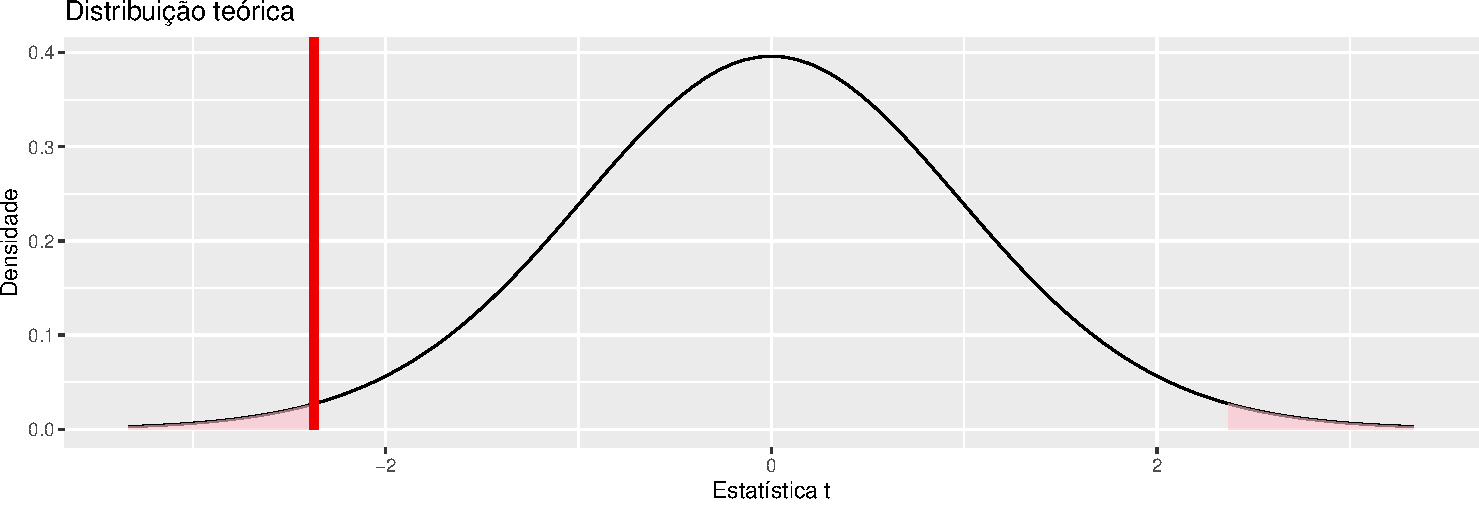
\includegraphics{aula_11_files/figure-beamer/unnamed-chunk-8-1.pdf}
\end{frame}

\begin{frame}[fragile]{Usando ggpubr}
\protect\hypertarget{usando-ggpubr}{}
\begin{Shaded}
\begin{Highlighting}[]
\KeywordTok{library}\NormalTok{(ggpubr)}
\NormalTok{dfe }\OperatorTok{\%\textgreater{}\%}\StringTok{ }\NormalTok{dplyr}\OperatorTok{::}\KeywordTok{filter}\NormalTok{(turma }\OperatorTok{\%in\%}\StringTok{ }\KeywordTok{c}\NormalTok{(}\StringTok{"3joan"}\NormalTok{,}\StringTok{"3joad"}\NormalTok{)) }\OperatorTok{\%\textgreater{}\%}\StringTok{ }
\StringTok{  }\KeywordTok{ggerrorplot}\NormalTok{(}\DataTypeTok{x =} \StringTok{"turma"}\NormalTok{, }\DataTypeTok{y =} \StringTok{"media"}\NormalTok{,}\DataTypeTok{color =} \StringTok{"turma"}\NormalTok{,}
              \DataTypeTok{position =} \KeywordTok{position\_dodge}\NormalTok{(}\FloatTok{0.5}\NormalTok{)) }\OperatorTok{+}
\StringTok{  }\KeywordTok{stat\_compare\_means}\NormalTok{(}\KeywordTok{aes}\NormalTok{(}\DataTypeTok{label =} \KeywordTok{paste0}\NormalTok{(..p.signif..,}\StringTok{" ou p = "}\NormalTok{, ..p.format..)),}
                     \DataTypeTok{method =} \StringTok{"t.test"}\NormalTok{) }\OperatorTok{+}\StringTok{ }\KeywordTok{theme}\NormalTok{(}\DataTypeTok{legend.position =} \StringTok{"right"}\NormalTok{)}
\end{Highlighting}
\end{Shaded}

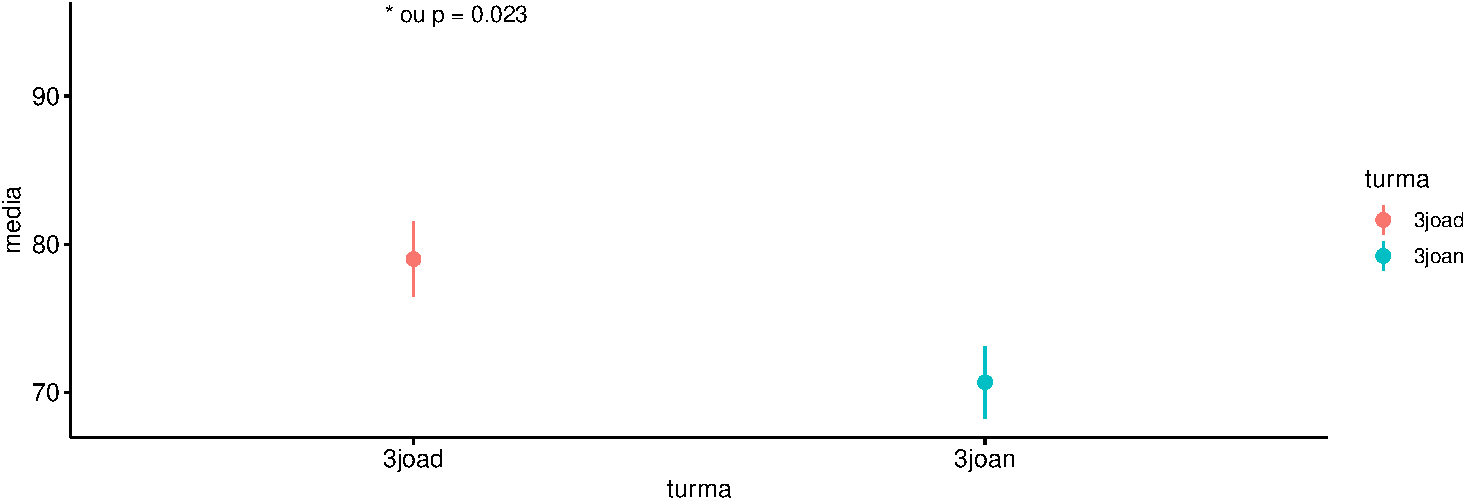
\includegraphics{aula_11_files/figure-beamer/unnamed-chunk-9-1.pdf}
\end{frame}

\begin{frame}[fragile]{Tamanho do efeito}
\protect\hypertarget{tamanho-do-efeito}{}
O d de Cohen pode ser usado como uma estatística de tamanho de efeito
para um teste t de duas amostras.

É calculado como a diferença entre as médias de cada grupo, dividido
pelo desvio padrão agrupado dos dados.

Um d de Cohen de 0,5 sugere que as médias diferem pela metade do desvio
padrão dos dados. Um d de Cohen de 1,0 sugere que as médias diferem por
um desvio padrão dos dados.

\begin{Shaded}
\begin{Highlighting}[]
\NormalTok{dfe }\OperatorTok{\%\textgreater{}\%}\StringTok{ }\NormalTok{dplyr}\OperatorTok{::}\KeywordTok{filter}\NormalTok{(turma }\OperatorTok{\%in\%}\StringTok{ }\KeywordTok{c}\NormalTok{(}\StringTok{"3joan"}\NormalTok{,}\StringTok{"3joad"}\NormalTok{)) }\OperatorTok{\%\textgreater{}\%}
\StringTok{  }\NormalTok{effectsize}\OperatorTok{::}\KeywordTok{cohens\_d}\NormalTok{(}\StringTok{"media"}\NormalTok{,}\StringTok{"turma"}\NormalTok{,}\DataTypeTok{data =}\NormalTok{ .)}
\end{Highlighting}
\end{Shaded}

\begin{verbatim}
Cohen's d |    1e+02% CI
------------------------
     0.77 | [0.10, 1.42]
\end{verbatim}
\end{frame}

\hypertarget{testando-diferentes-hipuxf3teses}{%
\section{Testando diferentes
hipóteses}\label{testando-diferentes-hipuxf3teses}}

\begin{frame}{Amostras pareadas}
\protect\hypertarget{amostras-pareadas}{}
Uma mesma medição em dois momentos no tempo para os mesmos indivíduos

\(H_0:\mu_{t2}-\mu_{t1}=0\) ou \(H_0:\mu_{\Delta}=0\)

\(H_A:\mu_{t2}-\mu_{t1}\neq0\) ou \(H_A:\mu_{\Delta}\neq0\)

Ex.:: Nota 1 e Nota 2
\end{frame}

\begin{frame}[fragile]{Com infer}
\protect\hypertarget{com-infer}{}
\begin{Shaded}
\begin{Highlighting}[]
\NormalTok{dif\_mu \textless{}{-}}\StringTok{ }\NormalTok{dfe }\OperatorTok{\%\textgreater{}\%}
\StringTok{  }\KeywordTok{mutate}\NormalTok{(}\DataTypeTok{d=}\NormalTok{nota2}\OperatorTok{{-}}\NormalTok{nota1) }\OperatorTok{\%\textgreater{}\%}
\StringTok{  }\KeywordTok{specify}\NormalTok{(}\DataTypeTok{response =}\NormalTok{ d) }\OperatorTok{\%\textgreater{}\%}
\StringTok{  }\KeywordTok{hypothesize}\NormalTok{(}\DataTypeTok{null =} \StringTok{"point"}\NormalTok{, }\DataTypeTok{mu =} \DecValTok{0}\NormalTok{) }\OperatorTok{\%\textgreater{}\%}
\StringTok{  }\KeywordTok{calculate}\NormalTok{(}\DataTypeTok{stat =} \StringTok{"t"}\NormalTok{)}

\NormalTok{hipotetica \textless{}{-}}\StringTok{ }\NormalTok{dfe }\OperatorTok{\%\textgreater{}\%}
\StringTok{  }\KeywordTok{mutate}\NormalTok{(}\DataTypeTok{d=}\NormalTok{nota2}\OperatorTok{{-}}\NormalTok{nota1) }\OperatorTok{\%\textgreater{}\%}
\StringTok{  }\KeywordTok{specify}\NormalTok{(}\DataTypeTok{response =}\NormalTok{ d) }\OperatorTok{\%\textgreater{}\%}
\StringTok{  }\KeywordTok{hypothesize}\NormalTok{(}\DataTypeTok{null =} \StringTok{"point"}\NormalTok{, }\DataTypeTok{mu =} \DecValTok{0}\NormalTok{) }\OperatorTok{\%\textgreater{}\%}
\StringTok{  }\KeywordTok{calculate}\NormalTok{(}\DataTypeTok{stat =} \StringTok{"t"}\NormalTok{)}
\end{Highlighting}
\end{Shaded}

\begin{Shaded}
\begin{Highlighting}[]
\NormalTok{hipotetica }\OperatorTok{\%\textgreater{}\%}\StringTok{ }\KeywordTok{visualize}\NormalTok{(}\DataTypeTok{method=}\StringTok{"theoretical"}\NormalTok{) }\OperatorTok{+}\StringTok{ }
\StringTok{  }\KeywordTok{shade\_p\_value}\NormalTok{(dif\_mu,}\DataTypeTok{direction=}\StringTok{"two{-}sided"}\NormalTok{) }\OperatorTok{+}
\StringTok{  }\KeywordTok{labs}\NormalTok{(}\DataTypeTok{title =} \StringTok{"Distribuição teórica"}\NormalTok{,}\DataTypeTok{x=}\StringTok{"Estatística t"}\NormalTok{,}\DataTypeTok{y=}\StringTok{"Densidade"}\NormalTok{)}
\NormalTok{dfe }\OperatorTok{\%\textgreater{}\%}\StringTok{ }\KeywordTok{mutate}\NormalTok{(}\DataTypeTok{d=}\NormalTok{nota2}\OperatorTok{{-}}\NormalTok{nota1) }\OperatorTok{\%\textgreater{}\%}\StringTok{  }\KeywordTok{t\_test}\NormalTok{(d }\OperatorTok{\textasciitilde{}}\StringTok{ }\OtherTok{NULL}\NormalTok{)}
\end{Highlighting}
\end{Shaded}
\end{frame}

\begin{frame}[fragile]{Visualizando}
\protect\hypertarget{visualizando-1}{}
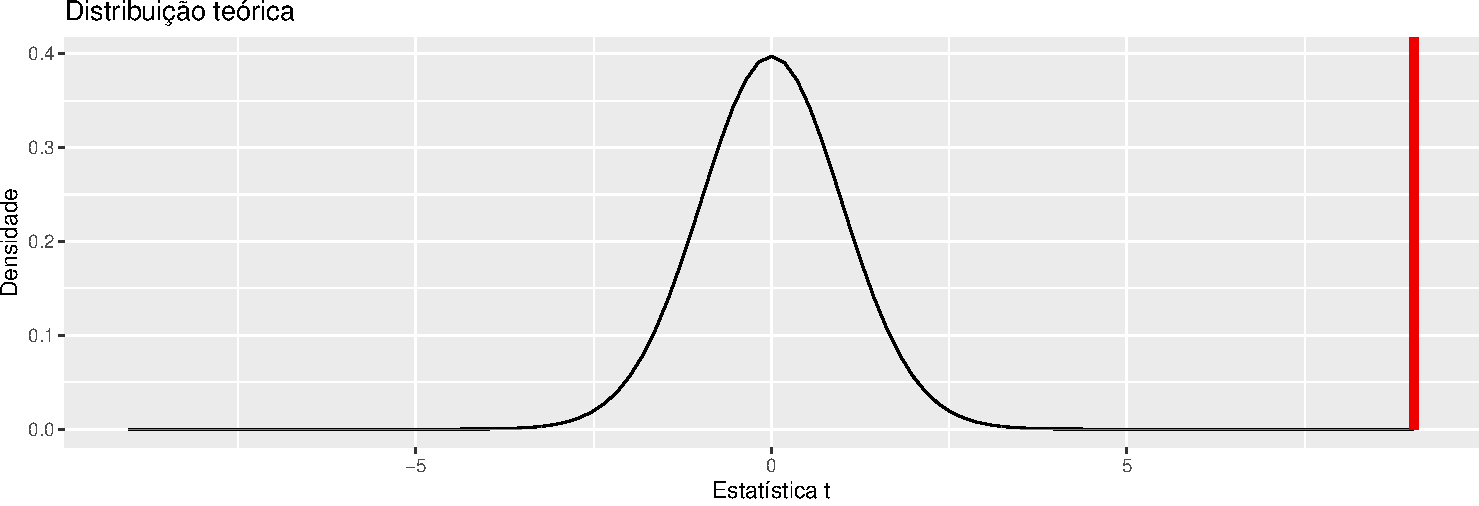
\includegraphics{aula_11_files/figure-beamer/unnamed-chunk-13-1.pdf}

\begin{verbatim}
# A tibble: 1 x 6
  statistic  t_df  p_value alternative lower_ci upper_ci
      <dbl> <dbl>    <dbl> <chr>          <dbl>    <dbl>
1      9.04    59 9.89e-13 two.sided       3.30     5.17
\end{verbatim}
\end{frame}

\begin{frame}{Por que ANOVA?}
\protect\hypertarget{por-que-anova}{}
\[
H_{0}: \mu_{1}=\mu_{2}=\cdots=\mu_{k}, \quad H_{A}: \mu_{i} \neq \mu_{j} \text{ para pelo menos um par } i \text{ e } j
\]
\end{frame}

\begin{frame}{O que é ANOVA?}
\protect\hypertarget{o-que-uxe9-anova}{}
Variabilidade dentro dos grupos = Soma dos Quadrados Dentro (SQD) \[
S Q D=\sum_{j=1}^{c} \sum_{i=1}^{n_{j}}\left(X_{i j}-\bar{X}_{j}\right)^{2}
\] Variabilidade entre grupos = Soma de Quadrados Entre (SQE)

\[
S Q E=\sum_{j=1}^{c} n_{j}\left(\bar{X}_{j}-\overline{\bar{X}}\right)^{2}
\] Variabilidade total = Soma Total de Quadrados (STQ)

\[
S T Q=\sum_{j=1}^{c} \sum_{i=1}^{n_{j}}\left(X_{i j}-\overline{\bar{X}}\right)^{2}
\]
\end{frame}

\begin{frame}{ANOVA}
\protect\hypertarget{anova}{}
\(\text{STQ} = \text{SQE} + \text{SQD}\)

Fração da variabilidade explicada pelo grupo =
\(\frac{\text{SQE}}{\text{STQ}}\)

É possível que, na população, as médias dos grupos sejam iguais e, por
acaso, as médias das amostras sejam diferentes.

Quanto maior a variabilidade entre grupos (SQE) e menor a variabilidade
dentro dos grupos (SQD), mais evidências teremos que as médias são
diferentes na população.

Princípio: Teste F:
\(\frac{\text{Variância entre grupos}}{\text{Variância dentro dos grupos}}\)

\(F = \frac{\text{MQE}}{\text{MQD}}\)
\end{frame}

\begin{frame}{Na prática}
\protect\hypertarget{na-pruxe1tica}{}
\(H_0:\text{A média de notas das turmas é igual}\) ou
\(H_0:\mu_\text{3joad}=\mu_\text{3joan}=\mu_\text{5joan}\)

\(H_A:\text{A média de notas de pelo menos uma das turmas é diferente}\)
ou \(H_A:\mu_\text{3joad} \neq \mu_\text{3joan} \neq \mu_\text{5joan}\)

Variável dependente: \textbf{Notas}

Variável independente: \textbf{Turma}
\end{frame}

\begin{frame}[fragile]{Função aov}
\protect\hypertarget{funuxe7uxe3o-aov}{}
\begin{Shaded}
\begin{Highlighting}[]
\NormalTok{ANOVAtest \textless{}{-}}\StringTok{ }\NormalTok{dfe }\OperatorTok{\%\textgreater{}\%}\StringTok{ }\KeywordTok{aov}\NormalTok{(.,}\DataTypeTok{formula =}\NormalTok{ media }\OperatorTok{\textasciitilde{}}\StringTok{ }\NormalTok{turma)}
\KeywordTok{summary}\NormalTok{(ANOVAtest)}
\end{Highlighting}
\end{Shaded}

\begin{verbatim}
            Df Sum Sq Mean Sq F value Pr(>F)  
turma        2    703   351.5   4.116 0.0214 *
Residuals   57   4867    85.4                 
---
Signif. codes:  0 '***' 0.001 '**' 0.01 '*' 0.05 '.' 0.1 ' ' 1
\end{verbatim}
\end{frame}

\begin{frame}[fragile]{Teste de Tukey}
\protect\hypertarget{teste-de-tukey}{}
\begin{Shaded}
\begin{Highlighting}[]
\NormalTok{Tt \textless{}{-}}\StringTok{ }\KeywordTok{TukeyHSD}\NormalTok{(ANOVAtest)}
\NormalTok{Tt}\OperatorTok{$}\NormalTok{turma }\OperatorTok{\%\textgreater{}\%}\StringTok{ }\KeywordTok{as.data.frame}\NormalTok{() }\OperatorTok{\%\textgreater{}\%}\StringTok{ }
\StringTok{  }\KeywordTok{rownames\_to\_column}\NormalTok{() }\OperatorTok{\%\textgreater{}\%}\StringTok{  }\KeywordTok{mutate}\NormalTok{(}\DataTypeTok{rowname =} \KeywordTok{gsub}\NormalTok{(}\StringTok{"}\CharTok{\textbackslash{}n}\StringTok{"}\NormalTok{,}\StringTok{""}\NormalTok{,rowname)) }\OperatorTok{\%\textgreater{}\%}
\StringTok{  }\NormalTok{knitr}\OperatorTok{::}\KeywordTok{kable}\NormalTok{(}\DataTypeTok{col.names =} \KeywordTok{c}\NormalTok{(}\StringTok{""}\NormalTok{,}\StringTok{"Dif."}\NormalTok{,}\StringTok{"Lim inf"}\NormalTok{,}\StringTok{"Lim sup"}\NormalTok{,}\StringTok{"p{-}valor"}\NormalTok{),}
               \DataTypeTok{digits=}\DecValTok{3}\NormalTok{,}\DataTypeTok{format =} \StringTok{"latex"}\NormalTok{)}
\end{Highlighting}
\end{Shaded}

\begin{tabular}{l|r|r|r|r}
\hline
 & Dif. & Lim inf & Lim sup & p-valor\\
\hline
3joan-3joad & -8.306 & -15.530 & -1.081 & 0.021\\
\hline
5joan-3joad & -5.818 & -12.689 & 1.052 & 0.112\\
\hline
5joan-3joan & 2.487 & -4.580 & 9.555 & 0.676\\
\hline
\end{tabular}
\end{frame}

\begin{frame}[fragile]{ANOVA com infer}
\protect\hypertarget{anova-com-infer}{}
\begin{Shaded}
\begin{Highlighting}[]
\NormalTok{observed\_f\_statistic \textless{}{-}}\StringTok{ }\NormalTok{dfe }\OperatorTok{\%\textgreater{}\%}\StringTok{ }
\StringTok{  }\KeywordTok{specify}\NormalTok{(media }\OperatorTok{\textasciitilde{}}\StringTok{ }\NormalTok{turma) }\OperatorTok{\%\textgreater{}\%}
\StringTok{  }\KeywordTok{calculate}\NormalTok{(}\DataTypeTok{stat =} \StringTok{"F"}\NormalTok{)}

\NormalTok{dfe }\OperatorTok{\%\textgreater{}\%}\StringTok{ }
\StringTok{  }\KeywordTok{specify}\NormalTok{(media }\OperatorTok{\textasciitilde{}}\StringTok{ }\NormalTok{turma) }\OperatorTok{\%\textgreater{}\%}
\StringTok{  }\KeywordTok{hypothesize}\NormalTok{(}\DataTypeTok{null =} \StringTok{"independence"}\NormalTok{) }\OperatorTok{\%\textgreater{}\%}
\StringTok{  }\KeywordTok{visualize}\NormalTok{(}\DataTypeTok{method =} \StringTok{"theoretical"}\NormalTok{) }\OperatorTok{+}\StringTok{ }
\StringTok{  }\KeywordTok{shade\_p\_value}\NormalTok{(observed\_f\_statistic,}
                \DataTypeTok{direction =} \StringTok{"greater"}\NormalTok{)}

\NormalTok{dfe }\OperatorTok{\%\textgreater{}\%}\StringTok{ }
\StringTok{  }\KeywordTok{specify}\NormalTok{(media }\OperatorTok{\textasciitilde{}}\StringTok{ }\NormalTok{turma) }\OperatorTok{\%\textgreater{}\%}
\StringTok{  }\KeywordTok{hypothesize}\NormalTok{(}\DataTypeTok{null =} \StringTok{"independence"}\NormalTok{) }\OperatorTok{\%\textgreater{}\%}
\StringTok{  }\KeywordTok{generate}\NormalTok{(}\DataTypeTok{reps =} \DecValTok{100}\NormalTok{, }\DataTypeTok{type =} \StringTok{"permute"}\NormalTok{) }\OperatorTok{\%\textgreater{}\%}
\StringTok{  }\KeywordTok{calculate}\NormalTok{(}\DataTypeTok{stat =} \StringTok{"F"}\NormalTok{) }\OperatorTok{\%\textgreater{}\%}
\StringTok{  }\KeywordTok{get\_p\_value}\NormalTok{(}\DataTypeTok{obs\_stat =}\NormalTok{ observed\_f\_statistic,}
              \DataTypeTok{direction =} \StringTok{"greater"}\NormalTok{)}
\end{Highlighting}
\end{Shaded}
\end{frame}

\begin{frame}[fragile]{}
\protect\hypertarget{section}{}
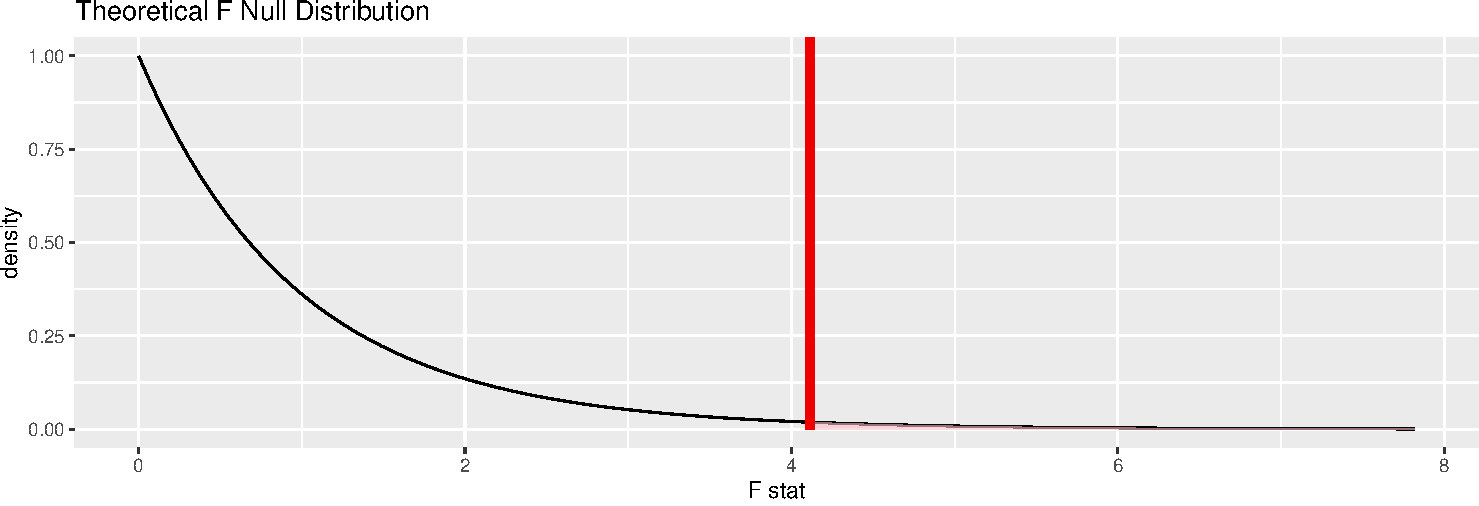
\includegraphics{aula_11_files/figure-beamer/unnamed-chunk-17-1.pdf}

\begin{verbatim}
# A tibble: 1 x 1
  p_value
    <dbl>
1    0.01
\end{verbatim}
\end{frame}

\begin{frame}[fragile]{Anova com ggpubr 1}
\protect\hypertarget{anova-com-ggpubr-1}{}
\begin{Shaded}
\begin{Highlighting}[]
\NormalTok{dfe }\OperatorTok{\%\textgreater{}\%}\StringTok{ }
\StringTok{ }\KeywordTok{ggboxplot}\NormalTok{(}\DataTypeTok{x =} \StringTok{"turma"}\NormalTok{, }\DataTypeTok{y =} \StringTok{"media"}\NormalTok{,}\DataTypeTok{color =} \StringTok{"turma"}\NormalTok{, }\DataTypeTok{palette =} \StringTok{"npg"}\NormalTok{)}\OperatorTok{+}
\StringTok{ }\KeywordTok{stat\_compare\_means}\NormalTok{(}\DataTypeTok{comparisons =} 
                      \KeywordTok{list}\NormalTok{(}\KeywordTok{c}\NormalTok{(}\StringTok{"3joad"}\NormalTok{,}\StringTok{"3joan"}\NormalTok{),}\KeywordTok{c}\NormalTok{(}\StringTok{"3joan"}\NormalTok{,}\StringTok{"5joan"}\NormalTok{),}\KeywordTok{c}\NormalTok{(}\StringTok{"3joad"}\NormalTok{, }\StringTok{"5joan"}\NormalTok{)), }
                    \DataTypeTok{label.y =} \KeywordTok{c}\NormalTok{(}\DecValTok{110}\NormalTok{, }\DecValTok{105}\NormalTok{, }\DecValTok{100}\NormalTok{))}\OperatorTok{+}\KeywordTok{stat\_compare\_means}\NormalTok{(}\DataTypeTok{label.y =} \DecValTok{120}\NormalTok{)    }
\end{Highlighting}
\end{Shaded}

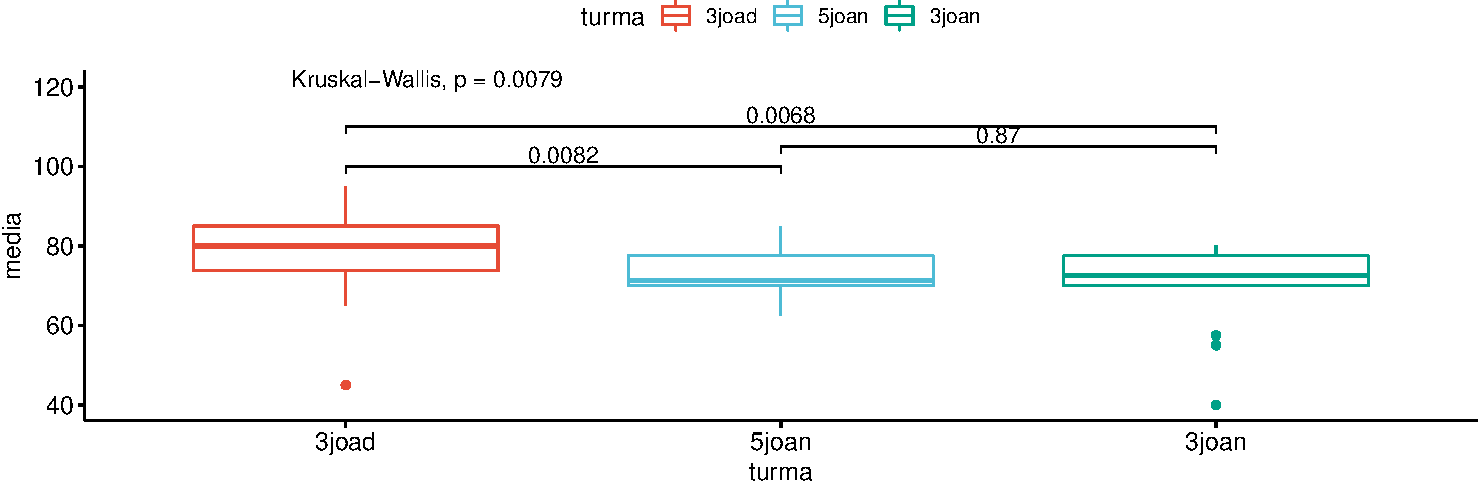
\includegraphics{aula_11_files/figure-beamer/unnamed-chunk-18-1.pdf}
\end{frame}

\begin{frame}[fragile]{Anova com ggpubr 2}
\protect\hypertarget{anova-com-ggpubr-2}{}
\begin{Shaded}
\begin{Highlighting}[]
\CommentTok{\# Multiple pairwise test against a reference group}
\NormalTok{dfe }\OperatorTok{\%\textgreater{}\%}\StringTok{ }
\StringTok{ }\KeywordTok{ggboxplot}\NormalTok{(}\DataTypeTok{x =} \StringTok{"turma"}\NormalTok{, }\DataTypeTok{y =} \StringTok{"media"}\NormalTok{,}\DataTypeTok{color =} \StringTok{"turma"}\NormalTok{, }\DataTypeTok{palette =} \StringTok{"npg"}\NormalTok{)}\OperatorTok{+}
\StringTok{ }\KeywordTok{stat\_compare\_means}\NormalTok{(}\DataTypeTok{method =} \StringTok{"anova"}\NormalTok{, }\DataTypeTok{label.y =} \DecValTok{120}\NormalTok{)}\OperatorTok{+}\StringTok{ }
\StringTok{ }\KeywordTok{stat\_compare\_means}\NormalTok{(}\KeywordTok{aes}\NormalTok{(}\DataTypeTok{label =}\NormalTok{ ..p.signif..),}\DataTypeTok{method =} \StringTok{"t.test"}\NormalTok{, }\DataTypeTok{ref.group =} \StringTok{"3joad"}\NormalTok{)}
\end{Highlighting}
\end{Shaded}

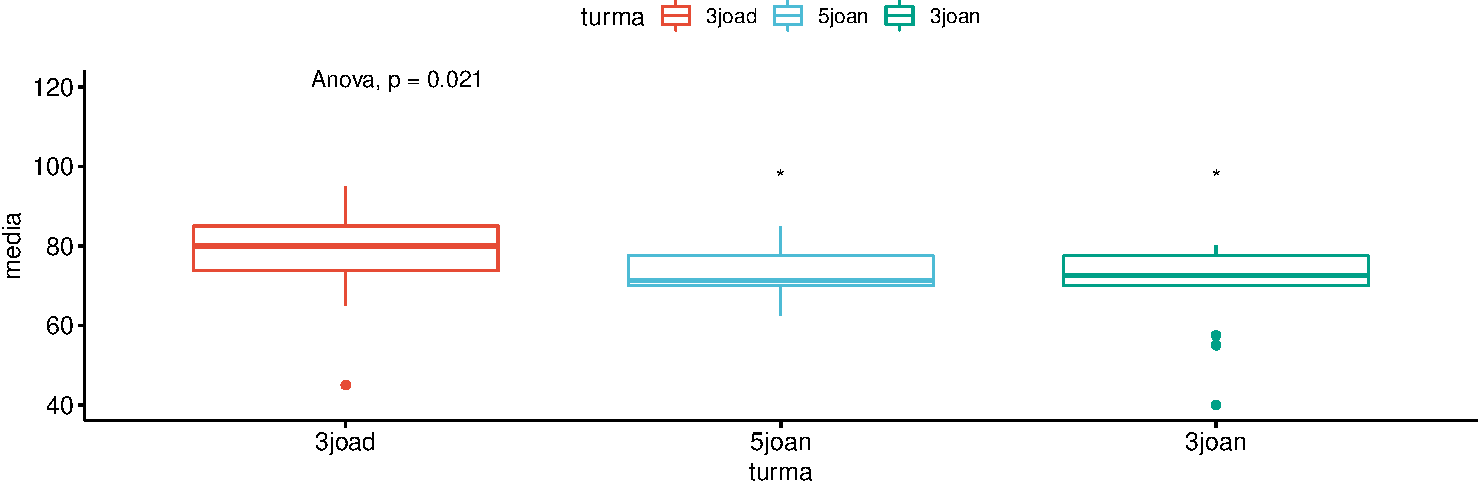
\includegraphics{aula_11_files/figure-beamer/unnamed-chunk-19-1.pdf}
\end{frame}

\begin{frame}[fragile]{Two-way ANOVA (dois fatores)}
\protect\hypertarget{two-way-anova-dois-fatores}{}
\begin{Shaded}
\begin{Highlighting}[]
\KeywordTok{summary}\NormalTok{(ANOVAtest2 \textless{}{-}}\StringTok{ }\NormalTok{dfe }\OperatorTok{\%\textgreater{}\%}\StringTok{ }\KeywordTok{aov}\NormalTok{(.,}\DataTypeTok{formula =}\NormalTok{ media }\OperatorTok{\textasciitilde{}}\StringTok{ }\NormalTok{turma }\OperatorTok{+}\StringTok{ }\NormalTok{interess))}
\end{Highlighting}
\end{Shaded}

\begin{verbatim}
            Df Sum Sq Mean Sq F value  Pr(>F)   
turma        2   1016   508.1   7.521 0.00131 **
interess     1      2     1.6   0.024 0.87840   
Residuals   54   3648    67.6                   
---
Signif. codes:  0 '***' 0.001 '**' 0.01 '*' 0.05 '.' 0.1 ' ' 1
2 observations deleted due to missingness
\end{verbatim}
\end{frame}

\begin{frame}[fragile]{Two-way ANOVA (dois fatores)}
\protect\hypertarget{two-way-anova-dois-fatores-1}{}
\begin{Shaded}
\begin{Highlighting}[]
\KeywordTok{library}\NormalTok{(agricolae); }\KeywordTok{HSD.test}\NormalTok{(ANOVAtest2, }\DataTypeTok{trt =} \KeywordTok{c}\NormalTok{(}\StringTok{"turma"}\NormalTok{,}\StringTok{"interess"}\NormalTok{),}\DataTypeTok{console =}\NormalTok{ T)}
\end{Highlighting}
\end{Shaded}

\begin{verbatim}
Study: ANOVAtest2 ~ c("turma", "interess")

HSD Test for media 

Mean Square Error:  67.5601 

turma:interess,  means

                    media       std  r  Min  Max
3joad:Principal  82.77778  9.052317  9 70.0 95.0
3joad:Secundário 78.88889  7.817360  9 65.0 90.0
3joan:Principal  68.95833 12.082027 12 40.0 80.0
3joan:Secundário 74.16667  4.082483  6 70.0 80.0
5joan:Principal  73.07692  4.466758 13 67.5 82.5
5joan:Secundário 73.33333  7.071068  9 62.5 85.0

Alpha: 0.05 ; DF Error: 54 
Critical Value of Studentized Range: 4.178265 

Groups according to probability of means differences and alpha level( 0.05 )

Treatments with the same letter are not significantly different.

                    media groups
3joad:Principal  82.77778      a
3joad:Secundário 78.88889     ab
3joan:Secundário 74.16667     ab
5joan:Secundário 73.33333     ab
5joan:Principal  73.07692     ab
3joan:Principal  68.95833      b
\end{verbatim}
\end{frame}

\begin{frame}[fragile]{Homogeneidade}
\protect\hypertarget{homogeneidade}{}
\begin{Shaded}
\begin{Highlighting}[]
\KeywordTok{plot}\NormalTok{(ANOVAtest2, }\DecValTok{1}\NormalTok{)}
\end{Highlighting}
\end{Shaded}

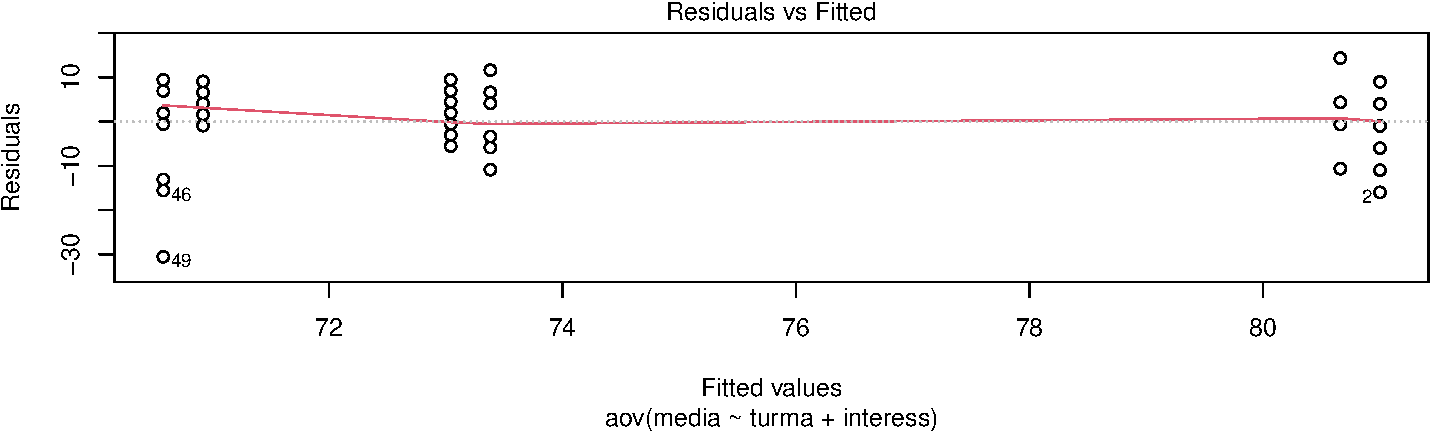
\includegraphics{aula_11_files/figure-beamer/unnamed-chunk-22-1.pdf}

\begin{Shaded}
\begin{Highlighting}[]
\KeywordTok{library}\NormalTok{(car);}\KeywordTok{leveneTest}\NormalTok{(media }\OperatorTok{\textasciitilde{}}\StringTok{ }\NormalTok{turma }\OperatorTok{*}\StringTok{ }\NormalTok{interess, }\DataTypeTok{data =}\NormalTok{ dfe)}
\end{Highlighting}
\end{Shaded}

\begin{verbatim}
Levene's Test for Homogeneity of Variance (center = median)
      Df F value Pr(>F)
group  5  0.8897 0.4948
      52               
\end{verbatim}
\end{frame}

\begin{frame}[fragile]{Normalidade}
\protect\hypertarget{normalidade}{}
\begin{Shaded}
\begin{Highlighting}[]
\KeywordTok{plot}\NormalTok{(ANOVAtest2,}\DecValTok{2}\NormalTok{); }\KeywordTok{shapiro.test}\NormalTok{(}\DataTypeTok{x =} \KeywordTok{residuals}\NormalTok{(}\DataTypeTok{object =}\NormalTok{ ANOVAtest2))}
\end{Highlighting}
\end{Shaded}

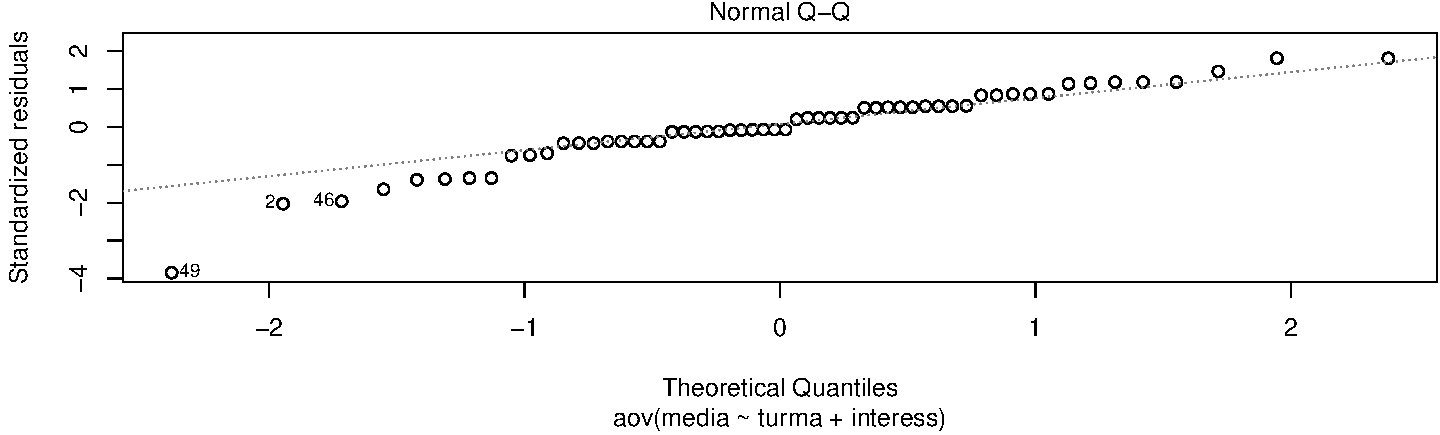
\includegraphics{aula_11_files/figure-beamer/unnamed-chunk-23-1.pdf}

\begin{verbatim}
    Shapiro-Wilk normality test

data:  residuals(object = ANOVAtest2)
W = 0.9331, p-value = 0.003273
\end{verbatim}
\end{frame}

\begin{frame}{Qui-quadrado}
\protect\hypertarget{qui-quadrado}{}
Vamos olhar as relações entre:

\begin{enumerate}
\item
  Estado civil e interesse na disciplina.
\item
  Interesse na disciplina e turma.
\end{enumerate}

Teste de independência entre variáveis categóricas.

\(H_0:\text{Variáveis são independentes}\)

\(H_A:\text{Variáveis não são independentes}\)
\end{frame}

\begin{frame}[fragile]{Tabelas de contingência e Qui-quadrado}
\protect\hypertarget{tabelas-de-continguxeancia-e-qui-quadrado}{}
Atenção à sua variável de interesse

\begin{Shaded}
\begin{Highlighting}[]
\NormalTok{dfe }\OperatorTok{\%\textgreater{}\%}\StringTok{ }\KeywordTok{drop\_na}\NormalTok{(estcivil,interess) }\OperatorTok{\%\textgreater{}\%}
\StringTok{  }\KeywordTok{tabyl}\NormalTok{(estcivil,interess)}
\end{Highlighting}
\end{Shaded}

\begin{verbatim}
 estcivil Secundário Principal
   Casado          5        12
 Solteiro         18        22
\end{verbatim}

\begin{Shaded}
\begin{Highlighting}[]
\NormalTok{dfe }\OperatorTok{\%\textgreater{}\%}\StringTok{ }\KeywordTok{drop\_na}\NormalTok{(estcivil,interess) }\OperatorTok{\%\textgreater{}\%}
\StringTok{  }\KeywordTok{tabyl}\NormalTok{(estcivil,interess) }\OperatorTok{\%\textgreater{}\%}\StringTok{ }
\StringTok{  }\NormalTok{janitor}\OperatorTok{::}\KeywordTok{adorn\_percentages}\NormalTok{(}\StringTok{"col"}\NormalTok{) }\OperatorTok{\%\textgreater{}\%}
\StringTok{  }\NormalTok{janitor}\OperatorTok{::}\KeywordTok{adorn\_pct\_formatting}\NormalTok{()}
\end{Highlighting}
\end{Shaded}

\begin{verbatim}
 estcivil Secundário Principal
   Casado      21.7%     35.3%
 Solteiro      78.3%     64.7%
\end{verbatim}
\end{frame}

\begin{frame}[fragile]{No infer}
\protect\hypertarget{no-infer}{}
\begin{Shaded}
\begin{Highlighting}[]
\NormalTok{qui\_quadrado \textless{}{-}}\StringTok{ }\NormalTok{dfe }\OperatorTok{\%\textgreater{}\%}\StringTok{ }\KeywordTok{drop\_na}\NormalTok{(estcivil,interess) }\OperatorTok{\%\textgreater{}\%}
\StringTok{   }\KeywordTok{mutate\_if}\NormalTok{(is.factor,as.character) }\OperatorTok{\%\textgreater{}\%}\StringTok{ }
\StringTok{  }\KeywordTok{specify}\NormalTok{(interess }\OperatorTok{\textasciitilde{}}\StringTok{ }\NormalTok{estcivil,}\DataTypeTok{success =} \StringTok{"Principal"}\NormalTok{) }\OperatorTok{\%\textgreater{}\%}
\StringTok{  }\KeywordTok{calculate}\NormalTok{(}\DataTypeTok{stat =} \StringTok{"Chisq"}\NormalTok{)}

\NormalTok{teorica\_qui\_quadrado \textless{}{-}}\StringTok{ }\NormalTok{dfe }\OperatorTok{\%\textgreater{}\%}\StringTok{ }\KeywordTok{drop\_na}\NormalTok{(estcivil,interess) }\OperatorTok{\%\textgreater{}\%}
\StringTok{  }\KeywordTok{mutate\_if}\NormalTok{(is.factor,as.character) }\OperatorTok{\%\textgreater{}\%}\StringTok{ }
\StringTok{  }\KeywordTok{specify}\NormalTok{(interess }\OperatorTok{\textasciitilde{}}\StringTok{ }\NormalTok{estcivil,}\DataTypeTok{success =} \StringTok{"Principal"}\NormalTok{) }\OperatorTok{\%\textgreater{}\%}
\StringTok{  }\KeywordTok{hypothesize}\NormalTok{(}\DataTypeTok{null =} \StringTok{"independence"}\NormalTok{) }
\end{Highlighting}
\end{Shaded}
\end{frame}

\begin{frame}[fragile]{Visualizando}
\protect\hypertarget{visualizando-2}{}
\begin{Shaded}
\begin{Highlighting}[]
\NormalTok{teorica\_qui\_quadrado  }\OperatorTok{\%\textgreater{}\%}
\StringTok{  }\KeywordTok{visualize}\NormalTok{(}\DataTypeTok{method =} \StringTok{"theoretical"}\NormalTok{) }\OperatorTok{+}\StringTok{ }
\StringTok{  }\KeywordTok{shade\_p\_value}\NormalTok{(qui\_quadrado,}
                \DataTypeTok{direction =} \StringTok{"greater"}\NormalTok{)}
\end{Highlighting}
\end{Shaded}

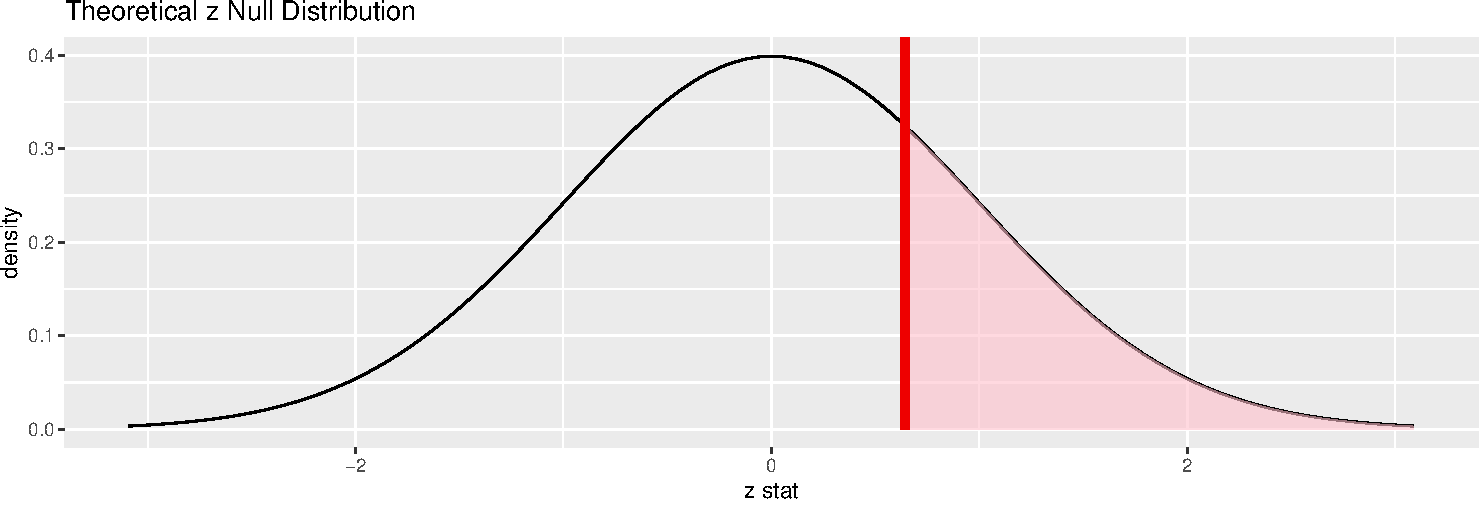
\includegraphics{aula_11_files/figure-beamer/unnamed-chunk-26-1.pdf}
\end{frame}

\begin{frame}[fragile]{O teste}
\protect\hypertarget{o-teste}{}
\begin{Shaded}
\begin{Highlighting}[]
\NormalTok{dfe }\OperatorTok{\%\textgreater{}\%}\StringTok{ }\KeywordTok{drop\_na}\NormalTok{(estcivil,interess) }\OperatorTok{\%\textgreater{}\%}
\StringTok{  }\KeywordTok{mutate}\NormalTok{(}\DataTypeTok{estcivil=}\KeywordTok{as.character}\NormalTok{(estcivil),}\DataTypeTok{interess=}\KeywordTok{as.character}\NormalTok{(interess)) }\OperatorTok{\%\textgreater{}\%}\StringTok{ }
\StringTok{  }\NormalTok{infer}\OperatorTok{::}\KeywordTok{chisq\_test}\NormalTok{(interess }\OperatorTok{\textasciitilde{}}\StringTok{ }\NormalTok{estcivil)}
\end{Highlighting}
\end{Shaded}

\begin{verbatim}
# A tibble: 1 x 3
  statistic chisq_df p_value
      <dbl>    <int>   <dbl>
1     0.644        1   0.422
\end{verbatim}
\end{frame}

\begin{frame}[fragile]{Tabelas de contingência e Qui-quadrado}
\protect\hypertarget{tabelas-de-continguxeancia-e-qui-quadrado-1}{}
\begin{Shaded}
\begin{Highlighting}[]
\NormalTok{dfe }\OperatorTok{\%\textgreater{}\%}\StringTok{ }\KeywordTok{drop\_na}\NormalTok{(turma,interess) }\OperatorTok{\%\textgreater{}\%}
\StringTok{  }\KeywordTok{tabyl}\NormalTok{(turma,interess)}
\end{Highlighting}
\end{Shaded}

\begin{verbatim}
 turma Secundário Principal
 3joad          9         9
 3joan          6        12
 5joan          9        13
\end{verbatim}
\end{frame}

\begin{frame}[fragile]{No infer}
\protect\hypertarget{no-infer-1}{}
\begin{Shaded}
\begin{Highlighting}[]
\NormalTok{qui\_quadrado \textless{}{-}}\StringTok{ }\NormalTok{dfe }\OperatorTok{\%\textgreater{}\%}\StringTok{ }\KeywordTok{drop\_na}\NormalTok{(turma,interess) }\OperatorTok{\%\textgreater{}\%}
\StringTok{  }\KeywordTok{mutate\_if}\NormalTok{(is.factor,as.character) }\OperatorTok{\%\textgreater{}\%}\StringTok{ }
\StringTok{  }\KeywordTok{specify}\NormalTok{(interess }\OperatorTok{\textasciitilde{}}\StringTok{ }\NormalTok{turma) }\OperatorTok{\%\textgreater{}\%}
\StringTok{  }\KeywordTok{calculate}\NormalTok{(}\DataTypeTok{stat =} \StringTok{"Chisq"}\NormalTok{)}

\NormalTok{teorica\_qui\_quadrado \textless{}{-}}\StringTok{ }\NormalTok{dfe }\OperatorTok{\%\textgreater{}\%}\StringTok{ }\KeywordTok{drop\_na}\NormalTok{(turma,interess) }\OperatorTok{\%\textgreater{}\%}
\StringTok{  }\KeywordTok{mutate\_if}\NormalTok{(is.factor,as.character) }\OperatorTok{\%\textgreater{}\%}\StringTok{ }
\StringTok{  }\KeywordTok{specify}\NormalTok{(interess }\OperatorTok{\textasciitilde{}}\StringTok{ }\NormalTok{turma) }\OperatorTok{\%\textgreater{}\%}
\StringTok{  }\KeywordTok{hypothesize}\NormalTok{(}\DataTypeTok{null =} \StringTok{"independence"}\NormalTok{) }
\end{Highlighting}
\end{Shaded}
\end{frame}

\begin{frame}[fragile]{Visualizando}
\protect\hypertarget{visualizando-3}{}
\begin{Shaded}
\begin{Highlighting}[]
\NormalTok{teorica\_qui\_quadrado }\OperatorTok{\%\textgreater{}\%}
\StringTok{  }\KeywordTok{visualize}\NormalTok{(}\DataTypeTok{method =} \StringTok{"theoretical"}\NormalTok{) }\OperatorTok{+}\StringTok{ }
\StringTok{  }\KeywordTok{shade\_p\_value}\NormalTok{(qui\_quadrado,}
                \DataTypeTok{direction =} \StringTok{"greater"}\NormalTok{)}
\end{Highlighting}
\end{Shaded}

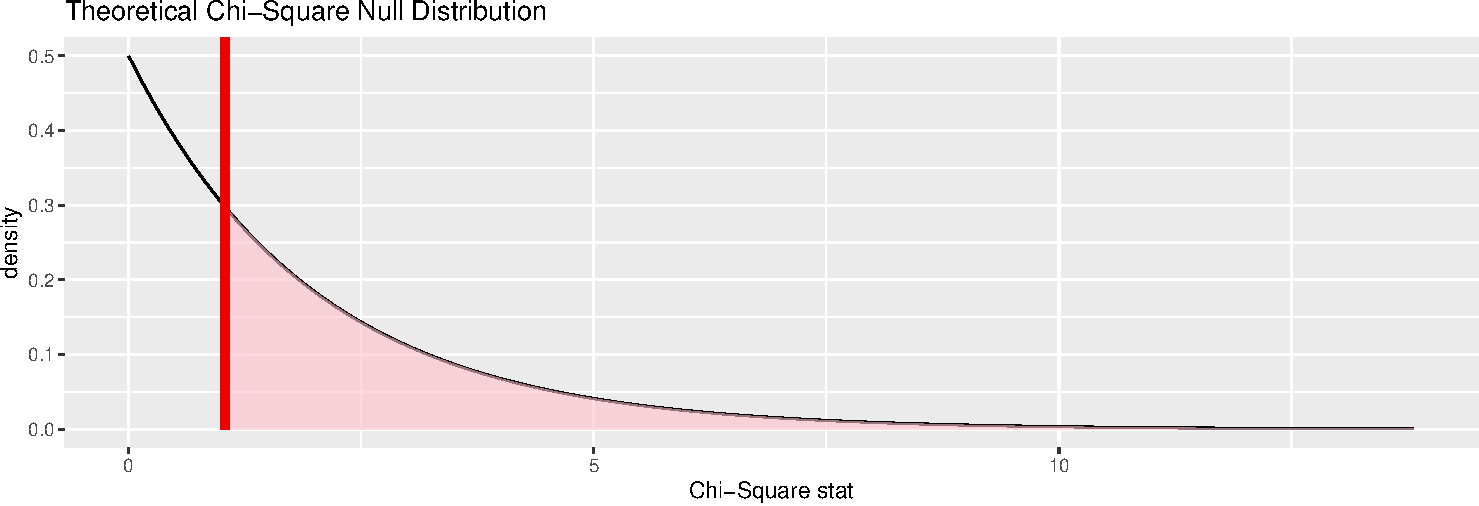
\includegraphics{aula_11_files/figure-beamer/unnamed-chunk-30-1.pdf}
\end{frame}

\begin{frame}[fragile]{O teste}
\protect\hypertarget{o-teste-1}{}
\begin{Shaded}
\begin{Highlighting}[]
\NormalTok{dfe }\OperatorTok{\%\textgreater{}\%}\StringTok{ }\KeywordTok{drop\_na}\NormalTok{(turma,interess) }\OperatorTok{\%\textgreater{}\%}
\StringTok{  }\KeywordTok{mutate\_if}\NormalTok{(is.factor,as.character) }\OperatorTok{\%\textgreater{}\%}\StringTok{ }
\StringTok{  }\KeywordTok{chisq\_test}\NormalTok{(turma }\OperatorTok{\textasciitilde{}}\StringTok{ }\NormalTok{interess) }
\end{Highlighting}
\end{Shaded}

\begin{verbatim}
# A tibble: 1 x 3
  statistic chisq_df p_value
      <dbl>    <int>   <dbl>
1      1.03        2   0.596
\end{verbatim}

\begin{Shaded}
\begin{Highlighting}[]
\NormalTok{dfe }\OperatorTok{\%\textgreater{}\%}\StringTok{ }\KeywordTok{drop\_na}\NormalTok{(turma,interess) }\OperatorTok{\%\textgreater{}\%}
\StringTok{  }\KeywordTok{mutate\_if}\NormalTok{(is.factor,as.character) }\OperatorTok{\%\textgreater{}\%}\StringTok{ }
\StringTok{  }\KeywordTok{chisq\_test}\NormalTok{(interess }\OperatorTok{\textasciitilde{}}\StringTok{ }\NormalTok{turma)}
\end{Highlighting}
\end{Shaded}

\begin{verbatim}
# A tibble: 1 x 3
  statistic chisq_df p_value
      <dbl>    <int>   <dbl>
1      1.03        2   0.596
\end{verbatim}
\end{frame}

\hypertarget{correlauxe7uxe3o}{%
\section{Correlação}\label{correlauxe7uxe3o}}

\begin{frame}{Correlação}
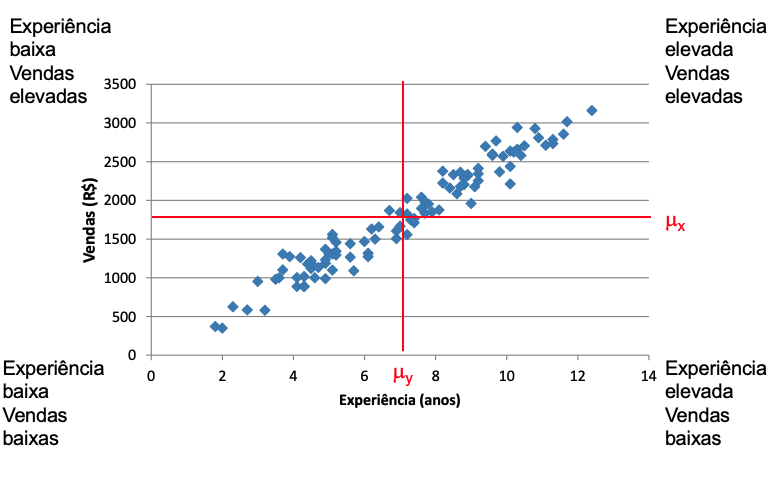
\includegraphics{imgs/corr1.png}
\end{frame}

\begin{frame}{}
\protect\hypertarget{section-1}{}
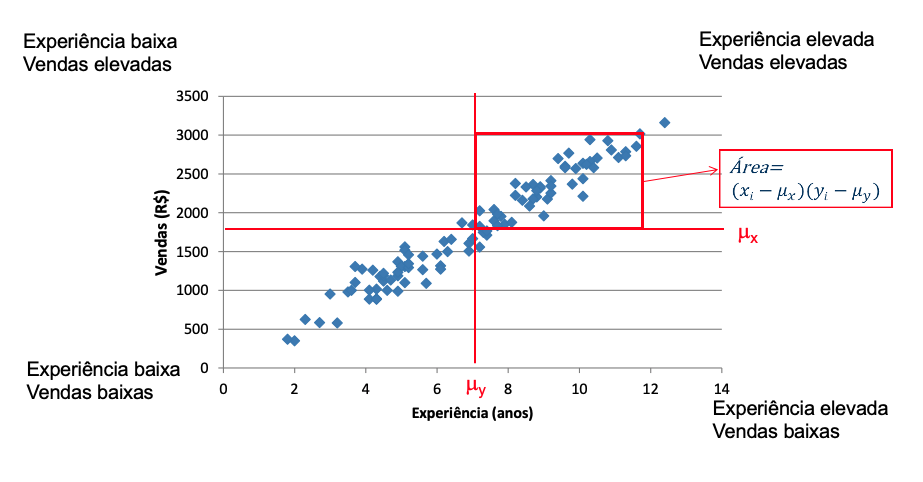
\includegraphics{imgs/corr2.png}
\end{frame}

\begin{frame}{}
\protect\hypertarget{section-2}{}
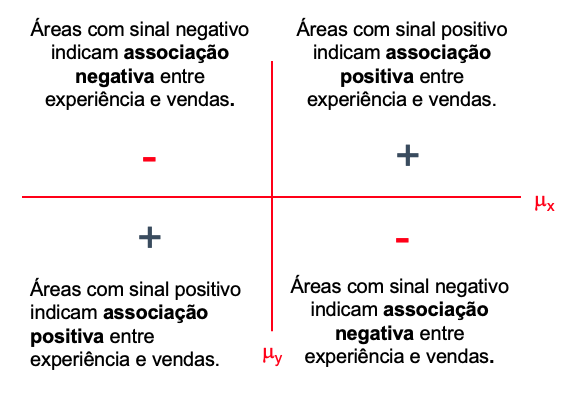
\includegraphics{imgs/corr3.png}
\end{frame}

\begin{frame}{}
\protect\hypertarget{section-3}{}
Três conceitos para a mesma idéia:

\begin{itemize}
\item
  Covariância
\item
  Correlação
\item
  Coeficiente de determinação (\(R^{2}\))
\end{itemize}

São grandes em valor absoluto se houver forte relação linear

\href{http://guessthecorrelation.com/}{Guess the correlation}
\end{frame}

\begin{frame}{Covariância e correlação}
\protect\hypertarget{covariuxe2ncia-e-correlauxe7uxe3o}{}
\[
\operatorname{Cov}(X, Y)=\frac{\sum_{i=1}^{N}\left(X_{i}-\mu_{x}\right)\left(Y_{i}-\mu_{y}\right)}{N}
\]

Uma área positiva indica associação positiva entre as variáveis.

\begin{itemize}
\item
  Mas como saber se é uma associação forte ou fraca?
\item
  Qual a unidade de medida da covariância?
\end{itemize}

Para eliminar a unidade de medida das variáveis, podemos usar a
padronização z. Desta forma, obtemos o coeficiente de correlação, que é
a covariância com variáveis padronizadas. Este coeficiente varia de -1 a
1.

\[
\operatorname{Corr}(X, Y)=\frac{\sum_{i=1}^{N}\left(\frac{X_{i}-\mu_{x}}{\sigma_{x}}\right)\left(\frac{Y_{i}-\mu_{y}}{\sigma_{y}}\right)}{N}
\]
\end{frame}

\begin{frame}{}
\protect\hypertarget{section-4}{}
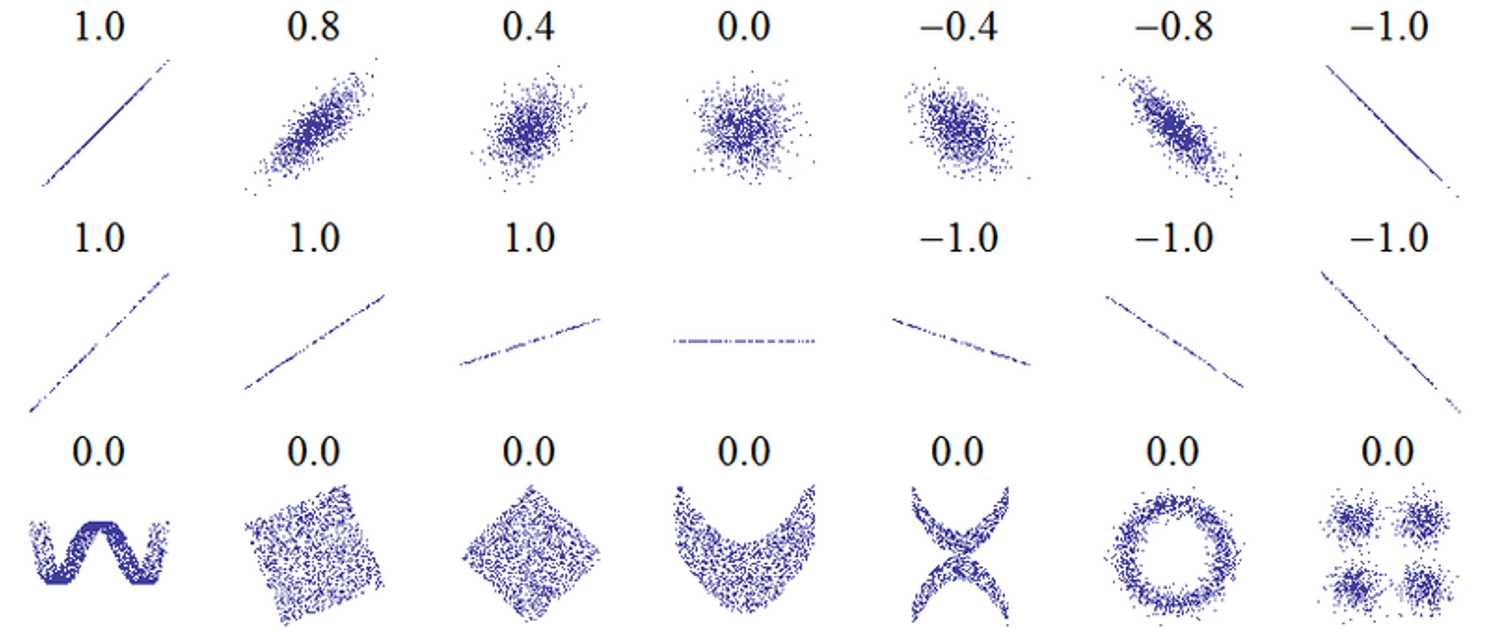
\includegraphics{imgs/correlacao.png}
\end{frame}

\begin{frame}[fragile]{Faltas e Nota 2}
\protect\hypertarget{faltas-e-nota-2}{}
\begin{Shaded}
\begin{Highlighting}[]
\NormalTok{dfe }\OperatorTok{\%\textgreater{}\%}\StringTok{ }\KeywordTok{ggplot}\NormalTok{(}\KeywordTok{aes}\NormalTok{(}\DataTypeTok{x=}\NormalTok{faltas,}\DataTypeTok{y=}\NormalTok{nota2)) }\OperatorTok{+}
\StringTok{  }\KeywordTok{geom\_point}\NormalTok{() }\OperatorTok{+}\StringTok{ }\KeywordTok{geom\_smooth}\NormalTok{(}\DataTypeTok{method=}\StringTok{"lm"}\NormalTok{)}
\end{Highlighting}
\end{Shaded}

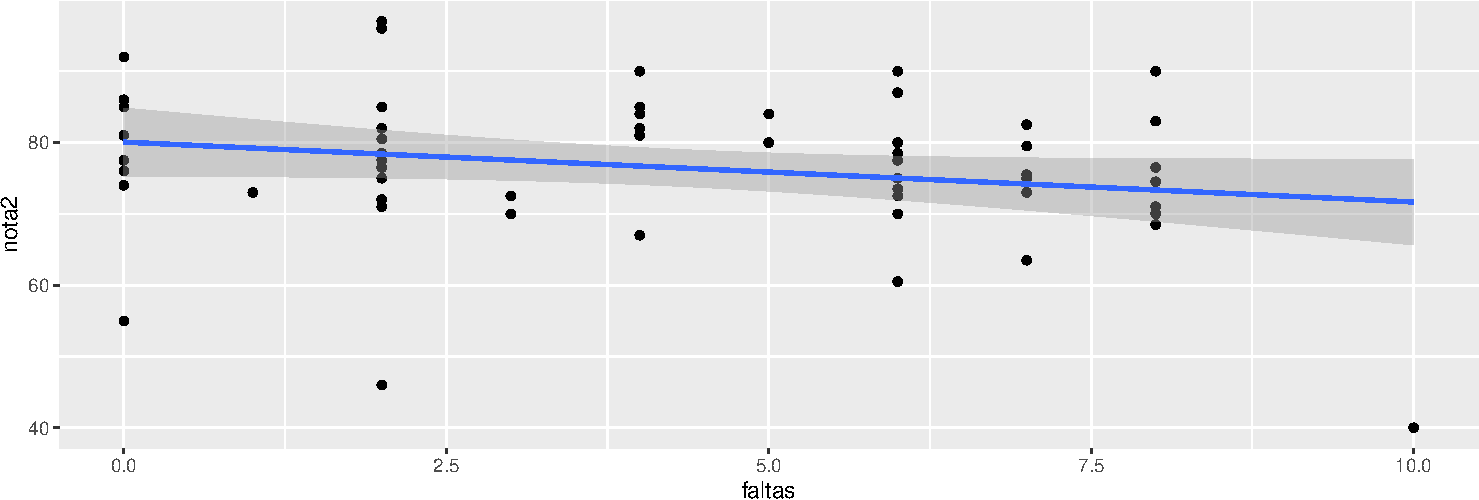
\includegraphics{aula_11_files/figure-beamer/unnamed-chunk-32-1.pdf}
\end{frame}

\begin{frame}[fragile]{Com ggpubr}
\protect\hypertarget{com-ggpubr}{}
\begin{Shaded}
\begin{Highlighting}[]
\NormalTok{dfe }\OperatorTok{\%\textgreater{}\%}\StringTok{ }\KeywordTok{ggscatter}\NormalTok{(}\DataTypeTok{x =} \StringTok{"faltas"}\NormalTok{, }\DataTypeTok{y =} \StringTok{"nota2"}\NormalTok{,}\DataTypeTok{add =} \StringTok{"reg.line"}\NormalTok{,}\DataTypeTok{conf.int =} \OtherTok{TRUE}\NormalTok{)}\OperatorTok{+}
\StringTok{  }\KeywordTok{stat\_cor}\NormalTok{(}\DataTypeTok{method =} \StringTok{"pearson"}\NormalTok{,}\DataTypeTok{label.x=}\DecValTok{7}\NormalTok{)}
\end{Highlighting}
\end{Shaded}

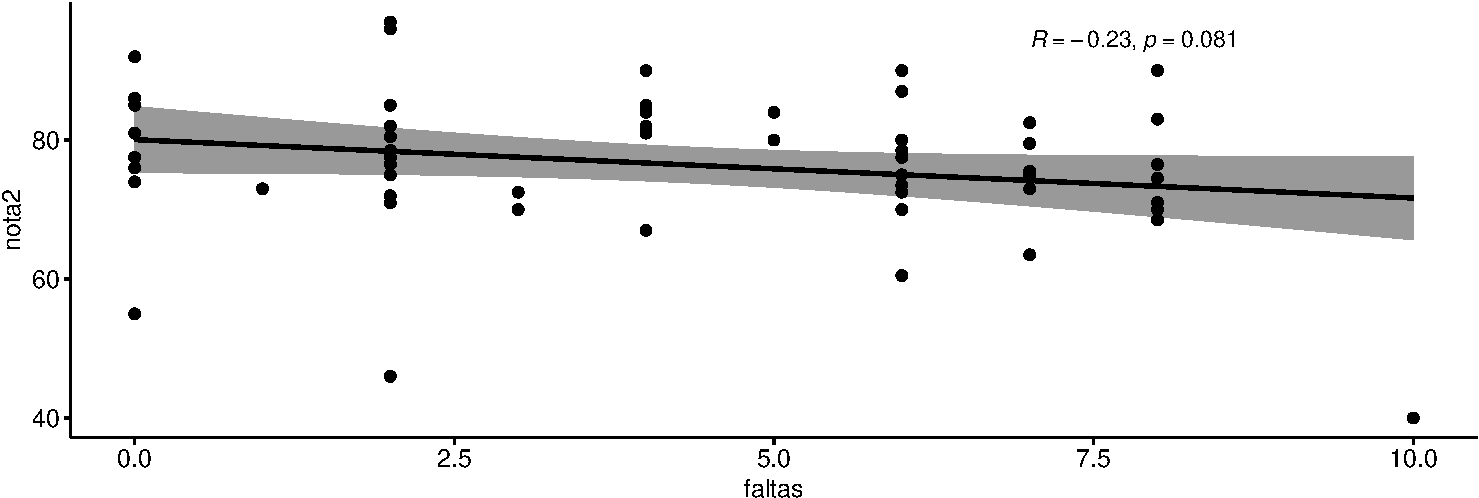
\includegraphics{aula_11_files/figure-beamer/unnamed-chunk-33-1.pdf}
\end{frame}

\begin{frame}[fragile]{Com ggpubr 2}
\protect\hypertarget{com-ggpubr-2}{}
\begin{Shaded}
\begin{Highlighting}[]
\NormalTok{dfe }\OperatorTok{\%\textgreater{}\%}\StringTok{ }\KeywordTok{ggscatter}\NormalTok{(}\DataTypeTok{x =} \StringTok{"faltas"}\NormalTok{, }\DataTypeTok{y =} \StringTok{"nota2"}\NormalTok{,}\DataTypeTok{add =} \StringTok{"reg.line"}\NormalTok{,}\DataTypeTok{conf.int =} \OtherTok{TRUE}\NormalTok{,}
          \DataTypeTok{color =} \StringTok{"turma"}\NormalTok{, }\DataTypeTok{palette =} \StringTok{"jco"}\NormalTok{,}\DataTypeTok{shape =} \StringTok{"turma"}\NormalTok{)}\OperatorTok{+}
\StringTok{  }\KeywordTok{stat\_cor}\NormalTok{(}\KeywordTok{aes}\NormalTok{(}\DataTypeTok{color =}\NormalTok{ turma), }\DataTypeTok{label.x =} \DecValTok{7}\NormalTok{,}\DataTypeTok{label.y=}\KeywordTok{c}\NormalTok{(}\DecValTok{110}\NormalTok{,}\DecValTok{105}\NormalTok{,}\DecValTok{100}\NormalTok{))}
\end{Highlighting}
\end{Shaded}

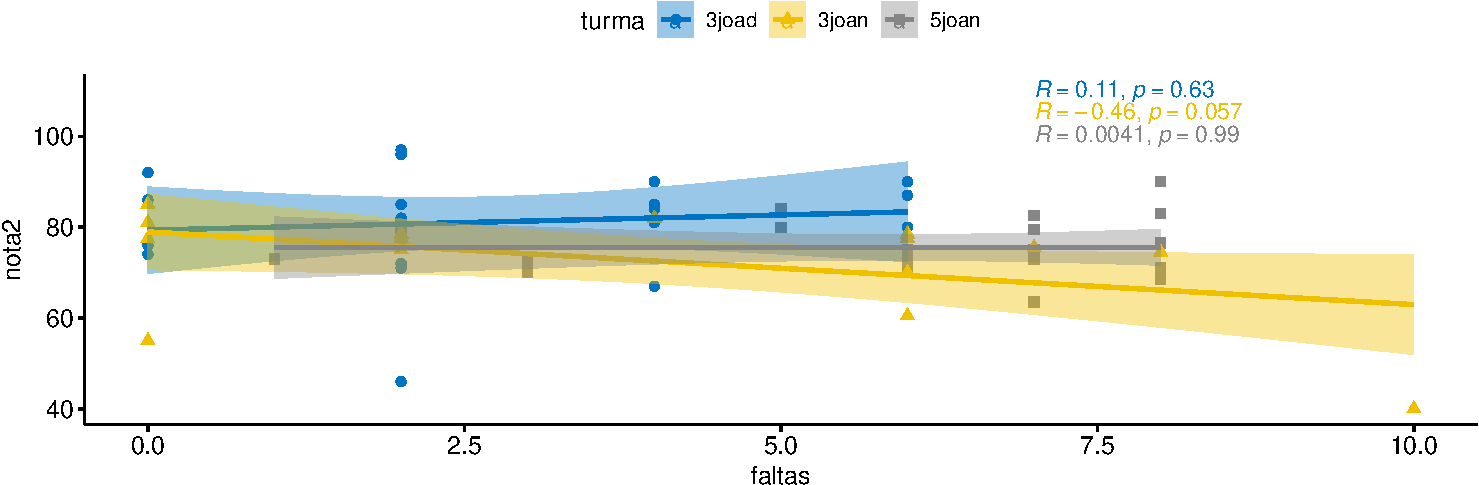
\includegraphics{aula_11_files/figure-beamer/unnamed-chunk-34-1.pdf}
\end{frame}

\begin{frame}[fragile]{Correlação}
\protect\hypertarget{correlauxe7uxe3o-1}{}
\href{http://www.sthda.com/english/wiki/correlation-analyses-in-r}{Um
bom Guia}

Vendo correlações graficamente

\begin{Shaded}
\begin{Highlighting}[]
\NormalTok{dfe }\OperatorTok{\%\textgreater{}\%}\StringTok{ }\KeywordTok{select\_if}\NormalTok{(is.numeric) }\OperatorTok{\%\textgreater{}\%}\StringTok{ }\KeywordTok{cor}\NormalTok{() }\OperatorTok{\%\textgreater{}\%}
\StringTok{  }\NormalTok{corrplot}\OperatorTok{::}\KeywordTok{corrplot}\NormalTok{(.,}\DataTypeTok{method=}\StringTok{"number"}\NormalTok{,}\DataTypeTok{type=}\StringTok{"upper"}\NormalTok{,}\DataTypeTok{diag=}\OtherTok{FALSE}\NormalTok{ )}
\end{Highlighting}
\end{Shaded}
\end{frame}

\begin{frame}{Vendo correlações graficamente}
\protect\hypertarget{vendo-correlauxe7uxf5es-graficamente}{}
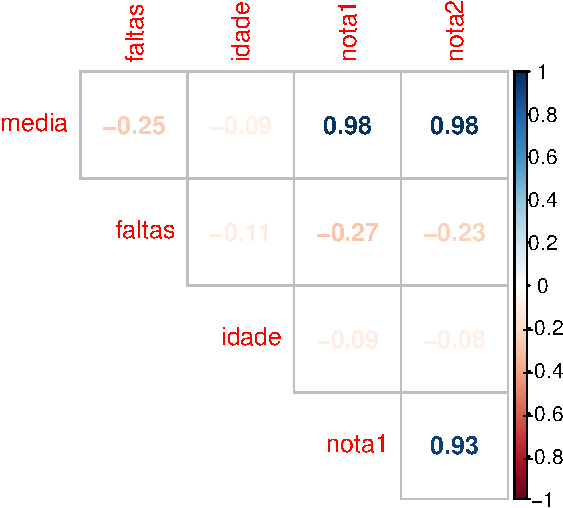
\includegraphics{aula_11_files/figure-beamer/unnamed-chunk-36-1.pdf}

\href{http://www.sthda.com/english/wiki/visualize-correlation-matrix-using-correlogram}{Para
mais}
\end{frame}

\hypertarget{modelo-linear-simples}{%
\section{Modelo Linear Simples}\label{modelo-linear-simples}}

\begin{frame}{Modelo Linear Simples}
\href{https://fmeireles.shinyapps.io/modelagem_r/}{Modelo linear simples
estimado por mínimos quadrados ordinários (MQO).}.
\end{frame}

\end{document}
